\documentclass[fr,license=none]{../../../eplsummary}

\usepackage{multirow}
\usepackage{wrapfig}
\usepackage{graphicx}
\usepackage{tabularx}
\usepackage{enumerate}

\usepackage{../../../eplcode}
\usepackage{../../../eplunits}

\hypertitle{Syst\`emes informatiques}{4}{SINF}{1252}
{Beno\^it Legat\and Damien Mercier}
{Olivier Bonaventure}

\lstset{language={C}}

\part{Le language \clang{}}
\section{Normes}
Depuis sa création par Dennis Ritchie,
le \clang{} a pas mal évolué.
Il existe plusieurs normes dont la norme \clang99 qui permet
de faire pas mal de nouvelles choses.

Pour demander à \lstinline[language=bash]|gcc|
de compiler du code avec \clang99,
il faut lui donner l'argument \lstinline[language=bash]|--std=c99|.

\section{Les pointeurs}
En \clang{}, les variables sont passées par \emph{valeur},
pour partager une variable sans la copier, on utilise les pointeurs.
Un pointeur contient l'adresse \emph{virtuelle} d'un endroit en mémoire.
\begin{lstlisting}
int n = 0;
int *i = &n;
printf("%d == n\n", *i, n); // imprime 0 == 0
\end{lstlisting}
On doit aussi donner ce vers quoi pointe l'adresse (ici, un \lstinline|int|)
pour permettre au compilateur d'effectuer de l'arithmétique de pointeur.
En effet, lorsqu'on fait
\begin{lstlisting}
int *p = 0x10;
p++;
\end{lstlisting}
\lstinline|p| n'est pas incrémenté de 1 mais de la taille d'un
\lstinline|int|, c'est à dire \lstinline|sizeof(int)|.

Par convention, \lstinline|NULL| est la valeur d'un pointeur qui
ne pointe pas encore vers de la mémoire allouée.
Il donc mieux toujours donner cette valeur à un pointeur qui ne pointe
pas vers quelque chose de telle sorte que
\begin{lstlisting}
if (p != NULL) {
  free(p);
}
\end{lstlisting}
ne libère jamais de la mémoire non-allouée

\subsection{Le heap}
Les pointeurs permettent aussi de s'allouer de la mémoire dans la \emph{heap}.
La heap est un endroit de la mémoire où on peut s'allouer dynamiquement
de la mémoire.
C'est à dire s'allouer un nombre de bytes
qu'on ne connait pas à la compilation.

Pour cela, on utilise la fonction \lstinline|malloc| qui alloue de la mémoire
et la fonction \lstinline|free| qui la libère.
En effet, si on ne libère jamais la mémoire qu'on s'alloue dans la heap,
elle risque d'être remplie et \lstinline|malloc| renverra alors
\lstinline|NULL|.
\lstinline|malloc| renvoie un pointeur de type \lstinline|void*|
pour rester générique.
Il faut le caster dans le type voulu.
\begin{lstlisting}
int n;
printf("Combien voulez-vous de int (%d bytes par int) ? : ",
       sizeof(int));
scanf("%d", &n);
// On s'alloue n int consecutifs dans la heap
int *p = (int*) malloc(n * sizeof(int));
if (p == NULL) {
  // n est negatif, nul ou trop grand
  printf("Vous avez ete un peut trop optimiste il me semble :)\n");
}
// utilisation de p
// On n'oublie pas de liberer la memoire
free(p);
p = NULL;
\end{lstlisting}

\lstinline|malloc| ne met pas de valeur dans la mémoire qu'elle alloue
et \lstinline|free| ne change pas la valeur de \lstinline|p|
(d'ailleurs il en est incapable car on ne lui a pas passé un pointeur
vers \lstinline|p|).

Il existe aussi la fonction \lstinline|calloc| qui contrairement à
\lstinline|malloc| initialise tous les bytes à 0.
\lstinline|calloc| est donc moins rapide que \lstinline|malloc| mais
met tous les bytes à 0 de manière très efficace.
\begin{lstlisting}
#define N 42
int *p = (int*) malloc(N * sizeof(int));
for (int i = 0; i < N; i++) {
  p[i] = 0;
}
// est plus lent que
int *p = (int*) calloc(N, sizeof(int));
\end{lstlisting}

\section{Structures}
On peut créer des structures qui des une sorte de classes sans méthodes.
On accède aux éléments à l'aide de \lstinline|.|, \lstinline|a.b|
est l'élément au label \lstinline|b| dans la variable \lstinline|a|.
On a un raccourcis pour \lstinline|(*a).b| qui est \lstinline|a->b|.
\begin{lstlisting}
struct point {
  int x;
  int y;
}
int move (struct point *p, struct point delta) {
  (*p).x += delta.x;
  p->y += delta.y;
}
int main () {
  struct point d;
  d.x = 1;
  d.y = 2;
  struct point *triangle = (struct point *) malloc(3 * sizeof(struct point));
  printf("Before\n");
  for (int i = 0; i < 3; i++) {
    triangle[i].x = i;
    triangle[i].x = i+1;
    printf("(%d, %d)\n", triangle[i].x, triangle[i].y);
  }
  printf("After\n");
  for (int i = 0; i < 3; i++) {
    move(triangle[i], d);
    printf("(%d, %d)\n", triangle[i].x, triangle[i].y);
  }
  free(triangle);
  return 0;
}
\end{lstlisting}

\section{Fonctions}
En \clang{}, les variables sont passées par \emph{valeur}.
Il n'y a jamais de passage par référence comme en \java{} pour les objets
ou comme pour le \oz{}.
Par exemple,
\begin{lstlisting}
void inc1 (int a) {
  a++;
}
void inc2 (int *b) {
  (*b)++;
}
void foo () {
  int n = 0;
  inc1(n);
  printf("%d\n", n); // affiche 0
  inc2(&n);
  printf("%d\n", n); // affiche 1
}
\end{lstlisting}
comme on fait un passage par valeur,
\lstinline|a| vaut 0 et changer \lstinline|a| ne change pas \lstinline|n|.
Par contre, \lstinline|b| contient l'adresse de \lstinline|n| donc modifier
\lstinline|*b| modifie bien \lstinline|n|.
C'est pour ça que pour \lstinline|scanf|,
il faut passer l'adresse de la variable qui doit stocker le résultat.

\section{Opérateurs}
\subsection{Opérateurs logiques}
Les opérateurs de bits s'exécutent sur chaque bits.
On a
\begin{center}
  \begin{tabular}{cccc}
    \clang{} bit & \clang{} \lstinline|bool| & Logique & Appelation\\
    \& & \&\& & $\land$ & and\\
    | & || & $\lor$ & or\\
    $\hat{}$ &  & $\oplus$ & xor
  \end{tabular}
\end{center}

\section{Portée des variables}
En \clang{}, il n'y a pas de classe,
les variables sont soient \emph{locales}, soient \emph{globales}.

\subsection{Variables globales}
Les variables globales sont initialisées à 0 ou NULL pour les pointeurs.
Elles sont visibles partout.
Elles sont déclarées à l'extérieur de toute fonction.

\subsection{Variables locales}
Elles ne sont pas initialisées.
Elles sont visibles uniquement à l'intérieur de la fonction à l'intérieur
de laquelle elles sont créées.
Si elles ont le même nom qu'une variable globales,
la variable globale ne sera pas disponible à l'intérieur de la fonction.
Contrairement aux variables globales, ces variables ne sont pas
initialisées.

\subsection{Variables de boucle}
À partir de la norme \clang99,
on peut déclarer des variables à l'intérieur
de n'importe quel bloc
\begin{lstlisting}
int main () {
  {
    int i = 0;
  }
  i = 1; // ne compile pas
  return 0;
}
\end{lstlisting}
ce qui permet d'écrire
\begin{lstlisting}
int main () {
  int sum = 0;
  for (int i = 0; i < 5; i++) {
    sum += i;
  }
  return 0;
}
\end{lstlisting}





\section{Types de données}
\subsection{Nombres entiers}
Les nombres sont limités par le nombre de bits qui sont utilisés pour les représentés en mémoire.
Il y deux types de nombres entiers : Les nombres entiers \textbf{signés} (\texttt{int}) et les nombres entiers \textbf{non-signés} (\texttt{unsigned int}).
\\
Par convention le bit le plus à gauche est appelé le \textbf{bit de poids fort} tandis que celui le plus à droite, est le \textbf{bit de poids faible}.
\\\\
Plusieurs représentations de séquence de bits existent : \\
\begin{tabular}{l||l|c|c|l}
  \textbf{Représentation} &  & \textbf{Base} & \textbf{Plage} & \textbf{Exemple} \\
  \hline \hline \textbf{Binaire} & Représente 1 bit & 2 & [0-1] & \texttt{0b1111011} \\
  \hline \textbf{Octal} & Représente 3 bits & 8 & [0-7] & \texttt{0x07b} \\
  \hline \textbf{Hexadécimal} & Représente 4 bits (nibble) & 16 & [0-9A-F] & \texttt{0173} \\
  \hline \textbf{Décimal} &  & 10 & [0-9] & \texttt{123} \\
  \hline
\end{tabular} \\
\begin{footnotesize}
  \textbf{Attention} : Lorsqu'on écrit un nombre commençant par un 0, le compilateur C le prendra comme étant en notation octale ! Donc \texttt{0123==123} renverra \texttt{false}, en effet, \texttt{\textbf{0}123} représente le nombre décimal \texttt{83}.

\end{footnotesize}
Afin de connaître la taille en mémoire d'un type de donnée en C, il faut utiliser \texttt{sizeof}.
\texttt{sizeof} renvoit le nombre d'\textbf{octet} (=8 bits)

\subsubsection{Nombres entiers signés}
Plusieurs manière existe pour représenter un nombre entier signé.
La première, consiste à utiliser le bit le plus à gauche afin de représenter le signe : $$ (-1)^{b_{n-1}} \times \sum_{i=0}^{n-2} b_i \times 2^i$$
En pratique, cette notation n'est que très peut utiliser car elle rend l'implémentation des circuits électroniques de calcul plus compliquée et qu'elle permet de représentée la valeur zéro de deux manière différentes : \texttt{00…00} et \texttt{10…00}

La représentation la plus courante est de sortir de la somme le bit de poids fort et de le multiplier par -1 :
$$ -(b_{n-1}) \times 2^{n-1} +  \sum_{i=0}^{n-2} b_i \times 2^i$$
De cette manière, il n'y a qu'une représentation pour le \texttt{0} (lorsque tout les bits valent \texttt{0}); par contre il existe toujours un nombre entier négatif qui n'a pas d'équivalent positif.

Un nombre \texttt{short} par exemple est représenté sur 16 bits, il peut donc représenter les nombres compris entre $-2^{15}$ et $2^{15} - 1$, c'est à dire les nombres entiers $\in [-32768, 32767]$.


Attention : Le langage C ne prévoit aucun mécanisme d'exception qui permettrait au programmeur de détecter qu'on dépasse l'intervalle autorisé pour un type de variable.
Il faut donc choisir le type de variable (\texttt{short}, \texttt{int}, \texttt{long}, \texttt{long long},...) judicieusement en fonction de l'application et être sûr qu'on ne dépasse pas l'intervalle.

\subsection{Nombres réels}
Pour un nombre réels sur 32 bits (resp 64 bits) on a : seeeeeeeemmmmmmmmmmmmmmmmmmmmmmm avec $s$ le signe sur 1 bit, $e$ l'exposant sur 8 bits (resp 11) et $m$ la fraction (ou mantise) sur 23 bits (resp 52)
$$(-1)^s\times(1+\sum^23_{i=1} m_i 2^{-i})\times 2^{e-E_{max}})$$
Il est intéressant de noter que
\begin{itemize}
  \item une représentation en virgule flottante sur $n$ bits ne permet jamais de représenter plus de $2^n$ nombres réels différents.
  \item les représentations en virgule flottante privilégient les nombres réels compris dans l'intervalle $[-1,1]$.
    On retrouve autant de nombres réels représentables dans cet intervalle qu'en dehors.
\end{itemize}

\subsection{Les tableaux}
En C, les tableaux permettent d'agréger des données d'un même type.
Exemple :
\begin{lstlisting}
#define N 10
int vecteur[N];
int matriceC[N][N];
int matriceR[N][2*N];
\end{lstlisting}

Attention : il n'est pas possible de récupérer la taille d'un tableau à partir de la variable (ex Java : coord1.length).
Il faut donc toujours passer cette information en plus du tableau (ex : \texttt{main(\textbf{int argc} , ...)}).

\subsection{Caractères et chaînes de caractères}
\subsubsection{Caractères}
Les caractères peuvent être encodé de plusieurs selon plusieurs représentations :
\begin{itemize}
  \item \textbf{ASCII} : 7 bits - mais représenté sur 8 bits.
    Par exemple "A" est 0b01000001.
  \item \textbf{ISO-8859} : 8 bits
  \item \textbf{Unicode} : Permet de représenter tous les caractères connus de toutes les langues.
    Utilise plus que 8 bits par caractères.
\end{itemize}
La fonction \texttt{toupper} prend un \texttt{int} comme argument et traite l'information en fonction du type d'encodage qui a été défini\footnote{Avec \texttt{setlocale}, voir \texttt{locale}}.

Dans la suite du cours, nous supposerons qu'un caractère est toujours représentable en utilisant le type \texttt{char} permettant de stocker un octet.

\subsubsection{Chaîne de caractères}
En C, les chaînes de caractères sont représentées sous forme de tableau de caractères (\texttt{char}).
Le dernier caractère d'une chaîne de caractère en C est par convention le caractère \texttt{$\backslash$0}.
Il faut faire attention à ne jamais le "dépasser" car le C n'a pas de mécanisme d'exception et donc aller trop loin dans le tableau ne produira pas d'exception du type \texttt{ArrayOutOfBoundException} mais un résultat imprévisible.


\subsection{Les pointeurs}
Un \textbf{pointeur} est définit comme étant une variable content l'adresse d'une autre variable.
\begin{lstlisting}
int i=1;				//entier
int *ptr_i;				//pointeur vers un entier

ptr_i=&i;				//initialisation du pointeur, a l'adresse de i
*ptr_i = *(ptr_i)+1252;	//Changement du contenu de la memoire pointe par ptr_i
\end{lstlisting}

\subsection{Les structures}
C Les structures permettent de définir des données plus complexes.
La langage C permet la définition de structures qui combinent différents types de données simples ou structurés.
Les structures permettent de facilement regrouper des données qui sont logiquement reliées entre elles et doivent être manipulées en même temps.
\begin{lstlisting}
// Definition d'une structure
struct student {
  int matricule ;
  char prenom [ 2 0 ] ;
  char nom [ 3 0 ] ;
};
// Declaration + Initialization
struct student linus = { 1 , "Linus" , "Torvalds" } ;
struct student richard = { .matricule = 2 , .prenom = "Richard" , .nom = "Stallman" } ;
struct student evil;
evil.noma = 3;
evil.prenom = "Bill";
evil.nom = "Gates ";
\end{lstlisting}


\texttt{typedef} permet de redéfinir le nom des types de données.
\begin{lstlisting}
// Definition de nouveaux noms pour des types existants
typedef int Entier;
typedef struct student Etudiant;
// Declaration de variable utilisant ces nouveaux noms
Entier matricule = 4;
Etudiant mark = {matricule , "Mark" , "Shuttleworth" };
\end{lstlisting}
Les données d'une structure peuvent être accédée via l'opérateur "\texttt{.}" (point).
Mais étant donnée que les pointeurs sont souvent utilisés lors de la manipulation de structures, une notation plus pratique que \texttt{(*ptr).elem} existe : \texttt{ptr->elem}.
\begin{lstlisting}
//Avec l'operateur '.'
printf("[%d] %s %s\n", mark.matricule, mark.nom, mark.prenom);
//Avec l'operateur '->'
Etudiant *e = &evil;
printf("[%d] %s %s\n" e->matricule, e->nom, e->prenom);
// qui est identique a :
printf("[%d] %s %s\n", (*e).matricule, (*e).nom, (*e).prenom);
\end{lstlisting}

\section{Compléments en langage C}
\subsection{Les fonctions}
\subsubsection{Déclaration \textit{vs} Définition}
La \textbf{déclaration} d'une fonction (= sa signature) indique au compilateur le type (en cas de variables) ou les arguments et le type de la valeur de retour (en cas de fonctions).
Toutes fonctions ou variables doivent être déclarée avant d'être utilisées.
En règle général, on regroupe toutes les déclarations de fonctions à l'intérieur d'un \textbf{fichier header} dont le nom se termine par \texttt{.h}

La \textbf{définition} d'une fonction consiste en l'implémentation de la fonction déclarée, ou dans le cas d'une variable de son initialisation.

\subsubsection{Passage des paramètres}
Le langage C utilise le \textbf{passage par valeur} des arguments.
Lorsqu'une fonction est exécutée, elle reçoit les valeurs de ces arguments.
Ces valeurs sont stockées dans une zone mémoire qui est locale à la fonction.
Toute modification faite sur la valeur d'une variable à l'intérieur d'une fonction est donc locale à cette fonction.
Attention néanmoins : Lorsqu'on passe un pointeur en argument on copie la valeur du pointeur (l'adresse d'une zone mémoire).
Le contenu de zone mémoire pointée par le pointeur n'est pas copié, il est donc possible à la fonction de le modifier\footnote{Cette remarque s'applique également aux tableaux, puisqu'un tableau un en réalité un pointeur}!
Par contre  si la fonction essaye de changer le pointeur lui même (pour qu'il pointe vers une autre zone mémoire) ce changement n'aura lieu que dans la fonction puisqu'il s'agit bien d'une copie du pointeur!


\subsection{Manipulation de bits}
Le langage C permet au programmeur de manipuler facilement les bits qui se trouves en mémoire.
Pour cela, le langage C définit des expressions qui correspondent à la plupart des opérations de manipulation de bits que l'on retrouve dans les langages d'assemblage.
Les premières opérations sont les opérations logiques, elles sont résumé par le tableau \ref{table:opbin}.

\begin{table}[!h]
  \begin{center}
    \begin{tabular}{|c|c||c|c|c|c|c}
      \hline
      \multirow{3}*{\textbf{A}} & \multirow{3}*{\textbf{B}} & \textit{négation} & \textit{conjonction logique} & \textit{disjonction logique} & \textit{ou exclusif} \\
                                & & \textbf{NOT(A)} & \textbf{A AND B} & \textbf{A OR B} & \textbf{A XOR B} \\
                                & & $\lnot A$ & $A \land B$ & $A \lor B$ & $A \oplus B$ \\
      \hline
      \hline 0 & 0 & \multirow{2}*{1} & 0 & 0 & 0 \\
      \cline{1-2}\cline{4-6} 0 & 1 &  & 0 & 1 & 1 \\
      \hline 1 & 0 & \multirow{2}*{0} & 0 & 1 & 1 \\
      \cline{1-2}\cline{4-6} 1 & 1 &  & 1 & 1 & 0 \\
      \hline \hline
      \multicolumn{6}{|l|}{\textbf{Exemple en C : }} \\
      \multicolumn{6}{|l|}{
        \begin{minipage}{0.5\textwidth}
          \texttt{char a = 0b01110011;}\\
          \texttt{char b = 0b00100101;}
        \end{minipage}
      } \\
      \hline
      \multicolumn{2}{|l|}{\textbf{Opération\footnotemark}} & \texttt{\~{}a} & \texttt{a\&b} & \texttt{a|b} & \texttt{a\^{}b} \\
      \hline
      \multicolumn{2}{|l|}{\textbf{Résultat}} & \texttt{0b10001100} & \texttt{0b00100001} & \texttt{0b01110111} & \texttt{0b01010110} \\
      \hline
    \end{tabular}
    \caption{Récapitulatif des opérations}
    \label{table:opbin}
  \end{center}
\end{table}
\footnotetext{Il faut faire attention à ne pas confondre les opérateurs binaires logique \texttt{\&} et \texttt{|} avec les expressions logique \texttt{\&\&} et \texttt{||} !}


Il est également important de mentionner les lois formulées par De Morgan qui peuvent se résumer par les équations suivantes :
$$\lnot ( A \lor B) = \lnot A \land \lnot B \text{~~~~~~~et~~~~~~~} \lnot ( A \land B) = \lnot A \lor \lnot B$$
Une des propriété intéressante de l'opération XOR est que $(A \oplus B) \oplus B = A$.
Cette propriété est largement utilisée par les méthodes de chiffrement.

\subsubsection{Décalage de bits}
\paragraph{Bit-shift à gauche} $n$ bits sont déplacés de B vers la gauche en ajoutant des 0 à droite.
En C : \texttt{a=n<<B}.
\paragraph{Bit-shift à droite} $n$ bits sont déplacés de B vers la droite en ajoutant des 0 à gauche.
En C : \texttt{a=n>>B}.
Ces opérations de décalage permettent différentes manipulations de bits\footnote{Pour un exemple, voir \texttt{int2bin} à la page 33 du syllabus [PDF]}.


\subsection{typecast en C}
Le langage C supporte des conversions implicites et explicites entre les différents types de données.
Ces conversions sont possibles entre les types primitifs et les pointeurs.
C'est régulièrement utilisé par exemple pour transformer un pointeur \texttt{void *} retourné par \texttt{malloc} en un pointeur du bon type.

Attention : Contrairement au compilateur Java, le compilateur C n'émet pas toujours de message de warning lors de l'utilisation de typecast qui risque d'engendrer une perte de précision.

\begin{lstlisting}[emph={unType,unAutreType,Etudiant},emphstyle={\color{blue}\bfseries}]
//Exemple de typecast
unType a = ... ;
unAutreType b = (unAutreType) a;

//Exemple concret
Etudiant * e;
e = (Etudiant*) malloc(sizeof(Etudiant));
\end{lstlisting}



\subsection{Les pointeurs}
En C, il est possible de définir des pointeurs vers n'importe quel type d'information qui est manipulé par un programme C.

Il est ainsi possible d'avoir des pointeurs vers des fonctions.
Cela peut être utile par exemple pour avoir une application qui propose différentes fonctions pour afficher (ou non) les informations de débogage.
Ou encore pour utiliser la fonction \texttt{qsort} qui permet de trier un tableau de n'importe quel type d'information.
Sa signature est la suivante : \\
\texttt{\textbf{void} qsort(\textbf{void} *base, \textbf{size\_t} nel, \textbf{size\_t} width, \textbf{int} (*compar) (\textbf{const void} *, \textbf{const void} *))}
Le quatrième argument est un pointeur vers la fonction qui permet de comparer deux élémets du tableau.
Cette fonction retourne un entier négatif si son premier argument est inférieur au second et positif ou nul sinon. \\

Il est également possible d'avoir des pointeurs vers des pointeurs.
En pratique, on retrouves des pointeurs vers des pointeurs lorsqu'on doit manipuler des structures multidimensionnelles, mais aussi lorsqu'il faut qu'une fonction puisse modifier une adresse qu'elle a reçue en argument\footnote{Comme par exemple la fonction \texttt{strtol} de la librairie standard qui prend comme 2e argument un pointeur vers une pointeur (\texttt{endptr}) qui permet d'indiquer un pointeur vers le premier caractère en erreur en cas d'erreur de conversion (sinon il indiquera le caractère de fin de chaîne \texttt{\\0}).}.

\subsection{Écriture de grands programme}
Lors de l'écriture de grands programme, il est préférable de les découper en modules.
Chaque module contient des fonctions qui traitent d'un même type de problème et sont fortement couplées.
Un module d'un programme C est en général décomposé en deux parties :
\begin{itemize}
  \item Le \textit{fichier header} : Contient les définitions de certaines constantes et les signatures des fonctions exportées par ce module.
    Ce fichier est en quelque sorte un résumé du module, c'est son interface externe.
    Il doit être inclus dans tout fichier qui utilise les fonctions du module\footnote{En pratique un fichier header ne peut être inclus qu'une seule fois.
      Mais comme il se peut qu'un fichier header fasse appel à un autre, on utilise la règle de bonne pratique suivante : On ajoute une condition au préprocesseur avec \texttt{\#ifndef \_MON\_MODULE\_} suivit de \texttt{\#define \_MON\_MODULE\_} en début de fichier header.
    On termine la condition avec \texttt{\#endif} en fin de fichier.}.
    Ce fichier contient donc :
    \begin{itemize}
      \item Signatures des fonctions.
        (Uniquement les fonctions qui sont destinées à être utilisées par des modules extérieures)
      \item Constantes qui sont utilisées à l'intérieur du module et doivent être visibles en dehors de celui-ci.
        Ces constantes peuvent être définie en utilisant des directives \texttt{\#define} du préprocesseur.
      \item Variables globales qui doivent être accessible en dehors du module.
    \end{itemize}
  \item Le fichier contenant le code du module.
\end{itemize}

Pour inclure des fichiers headers :
\begin{itemize}
  \item Soit il s'agit d'un module fournis par le système : \\
    \texttt{\#include <lemodule.h>}
  \item Soit il s'agit d'un module du programme (dans le même répertoire ou dans un répertoire définit en utilisant la variable d'environnement \texttt{GCC\_INCLUDE\_DIR} ou \texttt{CPATH}) : \\
    \texttt{\#include "lemodule.h"}
\end{itemize}
La procédure/ordre de compilation est expliqué dans le cours (page 90-91).


\subsection{\texttt{static}}
Le qualificateur \texttt{static} peut être utilisé dans différents cas :
\begin{itemize}
  \item Pour des variables définies en dehors d'un bloc dans un module : Dans ce cas, cette variable n'est accessible que par les fonctions du module.
  \item Pour des variables définies à l'intérieur d'un bloc (par exemple dans une fonction) : Dans ce cas, cela indique que cette variable doit toujours se trouver à la même localisation en mémoire, quelque soit le moment où elle est appelée.
    Ces variables sont placées par le compilateur dans le bas de la mémoire, avec les variables globales\footnote{Doit être utilisé avec beaucoup de précaution et bien documentées!}.
    Un de leurs intérête est qu'elles ne sont initialisées qu'au lancement du programme et non pas à chaque invocation de la fonction dans laquelle elles sont définies.
  \item Pour des fonctions : Lorsqu'une déclaration de fonction est précédée par le qualificateur \texttt{static}, cela indique que la fonction ne doit pas être visible en dehors du module dans lequel elle est définie.
\end{itemize}

\subsection{\texttt{extern}}
Lorsqu'une déclaration de variable globale est préfixée par \texttt{extern}, cela indique au compilateur que la variable est définie dans un autre module qui sera linké ultérieurement.
Le compilateur réserve une place pour cette variable dans la table des symboles du fichier objet, mais cette place ne pourra être liée à la zone mémoire qui correspond à cette variable que lorsque l'éditeur de liens combinera les différents fichiers objets entre eux.


\subsection{Traitement des erreurs}
Pour certaines fonctions ou appels systèmes, il est parfois nécessaire de fournir à l'utilisateur plus d'information sur l'erreur qui s'est produite.
La valeur de retour utilisée pour la plupart des fonctions de la librairie et appels système (souvent un \texttt{int} ou un pointeur), ne permet pas de fournir de l'information précise sur l'erreur qui s'est produite.

Les systèmes Unix utilisent la variable globale \texttt{errno} pour résoudre ce problème et permettre à une fonction de la librairie ou un appel système qui a échoué de donner plus de détails sur les raisons de l'échec.
Cette variable globale est définie dans \texttt{errno.h} qui doit être inclus par tout programme voulant tester ces codes d'erreur.
La librairie standard fournit également les fonctions \texttt{perror} et \texttt{strerror} qui facilitent l'écriture de messages d'erreur compréhensible pour l'utilisateur. \\
Attention : La valeur de \texttt{errno} n'est modifié qu'en cas d'échec, elle ne permet donc pas de savoir si une fonction a réussi ou non !



\section{Gestion et organisation de la mémoire}
\subsection{Déclarations et portées}
La \textbf{portée} d'une variable peut être définie comme étant la partie du programme où la variable est accessible et où sa valeur peut être modifiée.

En C, une variable a une \textbf{portée globale} lorsqu'elle est définie en dehors de toute définition de fonction.
Une telle variable est accessible dans toutes les fonctions présentes dans le fichier.
Dans un fichier donné, il ne peut donc évidemment pas y avoir deux variables globales qui ont le même identifiant.
Une variable définie dans un \textbf{bloc} a par contre une \textbf{portée locale} à ce bloc.
La variable n'existe pas avnt le début du bloc et n'existe plus à la fin du bloc.

Lorsqu'un identifiant de variable locale est utilisé à plusieurs endroits dans un fichier, c'est la définition la plus proche qui est utilisée.

En pratique, les variables globales doivent être utilisées de façon parcimonieuse et il faut limiter leur utilisation aux données qui doivent être partagées par plusieurs fonctions à l'intérieur d'un programme.
Lorsqu'une variable globale a été définie, il est préférable de ne pas réutiliser son identifiant pour une variable locale.

Les premières versions du langage C imposaient la définition de toutes les variables locales au début des blocs.
Les standards récents [C99] autorisent la déclaration de variables juste avant leur première utilisation ($\approx$ comme en Java).

\subsubsection{Constantes}
Les versions récentes de C [C99] permettent également de définir des variables dont la valeur sera constante durant toute l'exécution du programme.
Pour ce faire il faut utiliser le mot clé \texttt{const} devant la déclaration de la variable ($\approx$ \texttt{final} en Java).

Une autre façon de définir des constante est d'utiliser la macro \texttt{\#define} du préprocesseur qui permet de remplacer une chaîne de caractères par un nombre ou une autre chaîne de caractères.
Mais les inconvénients par rapport à \texttt{const} sont :
\begin{itemize}
  \item Avec \texttt{const} il est possible de définir n'importe quel type de données en C, y compris des structures ou des pointeurs.
    (Tandis qu'avec \texttt{\#define}, on ne peut définir que des nombres ou des chaînes de caractères.
  \item Les variables déclarée avec \texttt{const} sont stockées en mémoire, il est donc possible d'obtenir l'adresse en mémoire (pour l'examiner via un debugger par exemple).
\end{itemize}


\subsection{Organisation de la mémoire}
\begin{wrapfigure}{r}{0.3\textwidth}
  \vspace{-0.5cm}
  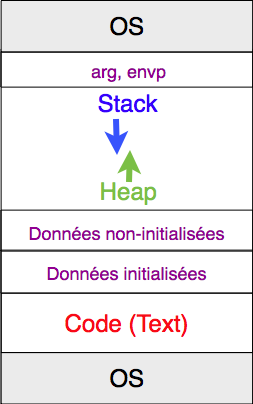
\includegraphics[width=0.3\textwidth]{mem}
  \caption{\label{fig:mem} Organisation d'un programme Linux en mémoire}
  \vspace{-2.5cm}
\end{wrapfigure}
Lorsqu'un programme s'exécute sur un système Unix, la mémoire peut être vue comme étant divisée en 6 zones principales (figure~\ref{fig:mem}).
\subsubsection{Le segment text}
La première zone est appelée le \textbf{\textit{segment text}}.
Elle est située dans la partie basse de la mémoire\footnote{Voir variable \textit{etext}}.
C'est dans cette zone que sont stockées toutes les instructions qui sont exécutées par le micro-processeur.
Elle est généralement considérée par l'OS comme étant uniquement accessible en lecture\footnote{Donc si un programme essaye de modifier son \textit{segment text} il sera immédiatement interrompu par le système d'exploitation}.
C'est dans le segment text q'un retrouvera les instructions de langage machine correspondant aux fonctions de calcul et d'affichage du programme.
$\Rightarrow$ langage d'assemblage.

\subsubsection{Le segment des données initialisées}
La deuxième zone appelée \textbf{\textit{segment des données initialisées}} contient l'ensemble des données et chaînes de caractères qui sont utilisées dans le programme.
Ce segment contient 2 types de données :
\begin{itemize}
  \item l'ensemble des variables globales qui sont explicitement initialisées par le programme ou initialisée à 0 par le compilateur.
  \item les constantes et chaînes de caractères utilisées par le programme.
\end{itemize}

\subsubsection{Le segment des données non-initialisées}
La troisième zone appelée \textbf{\textit{segment des données non-initialisées}} est réservée aux variables non initialisées.
Cette zone en mémoire est initialisée à zéro par l'OS au démarrage du programme.
C'est dans cette zone qu'on y stockera les valeurs de la variable \texttt{g} et des tableaux \texttt{array} et \texttt{msg} de l'exemple ci-dessous :

\begin{lstlisting}
#define MSG_LEN 10
int g;   // initialise par le compilateur
int g_init=1252;
const int un=1;
int tab[3]={1,2,3};
int array[10000];
char cours[]="SINF1252";
char msg[MSG_LEN]; // initialise par le compilateur

int main(int argc, char *argv[]) {
  int i;
  printf("g est a l'adresse %p et initialisee a %d\n",&g,g);
  printf("msg est a l'adresse %p contient les caracteres :",msg);
  for(i=0;i<MSG_LEN;i++)
  printf("%x ",msg[i]);
  printf("\n");
  printf("Cours est a l'adresse %p et contient : %s \n",&cours,cours);
  return(EXIT_SUCCESS);
}
\end{lstlisting}


\paragraph{Initialisation des variables} En C, il faut être attentif a bien initialiser l'ensemble des variables utilisées dans un programme car le compilateur C est très permissif (contrairement au compilateur Java).
Le compilateur C n'initialise pas les variables locales à zéro (pour un gain de performance), on ne peut donc pas faire d'hypothèse sur la valeur d'une variable non initialisée.

\subsubsection{Le tas (ou heap)}
La quatrième zone de la mémoire est le \textbf{\textit{tas}} (ou \textit{heap}).
Il s'agit d'une des deux zone dans laquelle un programme peut obtenir de la mémoire supplémentaire pour stocker de l'information.
L'OS mémorise pour chaque processus en cours d'exécution, la limite supérieure de son \textit{heap}.
Et permet à un processus de modifier la taille de son heap via les appels systèmes \texttt{brk} et \texttt{sbrk}.
Ces deux appels systèmes sont rarement utilisé directement car ils se contentent uniquement de modifier la limite supérieure du heap sans fournir d'API permettant d'y allouer efficacement des blocs de mémoire\footnote{On peut néanmoins utiliser directement \texttt{brk} sous forme d'un appel à \texttt{sbrk(0)} de façon à connaître la limite supérieure actuelle du heap}.

\paragraph{\texttt{malloc} et \texttt{free}}

En C, la plupart des processus allouent et libèrent de la mémoire en utilisant les fonctions \texttt{malloc} et \texttt{free} qui font partie de la librairie standard.

La fonction \texttt{malloc} prend comme argument la taille (en bytes) de la zone mémoire à allouer.
Cette taille doit être de type \texttt{size\_t}, il est important de toujours utiliser \texttt{sizeof} lors du calcul de la taille d'une zone mémoire à allouer.
\texttt{malloc} retourne un pointeur du type \texttt{(void *)} qui peut être casté en un pointeur du bon type.

La fonction \texttt{free} permet quant à elle de libérer la mémoire qui a été allouée par \texttt{malloc}.
Elle prend comme argument le pointeur dont la valeur a été initialisée par \texttt{malloc}.
La valeur du pointeur n'est pas modifiée, mais après libération de la mémoire il n'est évidemment plus permit d'accéder aux données qui étaient stockées dans cette zone\footnote{Bien que le compilateur C ne génère pas de code permettant de vérifier automatiquement qu'un accès via un pointeur pointe ou non vers une zone mémoire qui est libre (pour des raisons de performance).}.

\texttt{malloc} et \texttt{free} sont fréquemment utilisés dans des programmes qui manipulent des structures de données dont la taille varie dans le temps.
C'est le cas par exemple pour les différentes sortes de listes chaînées, les piles, les queues, les arbres,...

Attention : Il ne faut pas compter sur les \texttt{free} implicite.
Lorsqu'un programme se termine, via \texttt{return} dans la fonction \texttt{main} ou par un appel explicite à \texttt{exit}, l'OS libère tous les segments utilisés par le programme, le text, les données, le tas et la pile.
Néanmoins, ne pas libérer la mémoire lorsqu'elle n'est plus utilisée est un problème courant qui est généralement baptisé \textit{memory leak}.
Ce problème est particulièrement gênant pour les processus tels que les serveurs Internet qui ne se terminent pas ou des processus s'exécutant longtemps.
Une petite erreur de programmation causant un \texttt{memory leak} peut après quelque temps consommer une grande partie de l'espace mémoire inutilement.
Ce n'est pas acceptable !

Il existe également d'autres fonctions que \texttt{malloc} et \texttt{free} dans la librairie standard.
Citons \texttt{calloc} qui permet d'initialiser la mémoire à 0\footnote{Il est aussi possible d'initialiser la mémoire avec \texttt{memset} ou \texttt{bzero}}.

\subsubsection{Les arguments et variables d'environnement}
La zone situé dans le haut de la mémoire est une zone qui contient deux type de variables :
\begin{itemize}
  \item Les arguments qui ont été passés via la ligne de commande.
    L'OS met dans \texttt{argc} le nombre d'arguments et place dans \texttt{char *argv[]} tous les arguments passés avec dans \texttt{argv[0]} le nom du programme qui est exécuté.
  \item Ensuite les variables d'environnement.
\end{itemize}

\paragraph{Les variables d'environnements}
Ces variables sont généralement relatives à la configuration du système.
Leurs valeurs sont définies par l'administrateur système ou l'utilisateur.
De nombreuses variables d'environnement sont utilisées dans les système Umix.
Elles servent à modifier le comportement de certains programmes.
Voici quelques variables utiles\footnote{Il est possible de lister les définitions actuelles des variables d'environnement via la commande \texttt{printenv}.
  Les interpréteurs de commande tels que bash permettent de facilement modifier les valeurs de ces variables.
La plupart d'entre elles sont initialisées par le système ou via les fichiers qui sont chargés automatiquement au démarrage de l'interpréteur comme le fichier \texttt{/etc/profile} et le fichier \texttt{.profile} du répertoire utilisateur.}

\noindent\begin{tabularx}{\textwidth}{|p{0.08\textwidth}|p{0.45\textwidth}|p{0.05\textwidth}p{0.1\textwidth}|p{0.185\textwidth}|}
  \hline
  \textbf{Nom} & \textbf{Description} & \multicolumn{2}{c|}{\textbf{Définit par}} & \textbf{Exemple} \\
  \hline \hline
  \texttt{HOSTNAME} & Nom de la machine sur laquelle le programme s'exécute.
  & Admin & \texttt{hostname} & \texttt{damien-laptop}\\
  \hline
  \texttt{SHELL} & Interpréteur de commande utilisé par défaut pour l'utilisateur courant.
  Cet interpréteur est lancé par le système au démarrage d'une session de l'utilisateur.
  Il est stocké dans le fichier des mots de passe.
  & User & \texttt{passwd} & \texttt{/bin/bash} \\
  \hline
  \texttt{USER} & Nom de l'utilisateur courant.
  Sous Unix, chaque utilisateur est identifié par un numéro d'utilisateur et un nom uniques.
  & Admin & \texttt{passwd} & \texttt{damien} \\
  \hline
  \texttt{HOME} & Répertoire d'accueil de l'utilisateur courant.
  Ce répertoire d'accueil appartient à l'utilisateur.
  C'est dans ce répertoire qu'il peut stocker tous ses fichiers.
  & & & \texttt{/home/damien} \\
  \hline
  \texttt{PRINTER} & Nom de l'imprimante par défaut qui est utilisé par \texttt{lp} & & & \\
  \hline
  \texttt{PATH} & Contient la liste ordonnée des répertoires que le système parcourt pour trouver un programme à exécuter.
  Cette liste contient généralement les répertoires dans lesquels le système stocke les exécutables standards ainsi que des répertoires relatifs à des programmes spécialisés\footnote{Par exemple \texttt{/usr/lib/mozart/bin}}.
  & User\footnote{par exemple en ajoutant \texttt{PATH=\$PATH : \$HOME/local/bin : .} dans le fichier \texttt{.profile}.
Dans cet exemple le répertoire \texttt{\~{}/local/bin} sera ajouté ainsi que le répertoire courant symbolisé par le "\texttt{.}".} & & \texttt{/usr/local/sbin: /usr/local/bin: /usr/sbin: /usr/bin: /sbin: /bin: /usr/games}\\
  \hline
\end{tabularx}

La librairie standard contient plusieurs fonctions qui permettent de manipuler les variables d'environnement d'un processus.
\begin{itemize}
  \item \texttt{getenv} permet de récupérer la valeur associée à une variable d'environnement.
    Retourne un pointeur \texttt{NULL} si la variable n'a pas été assignée.
  \item \texttt{unsetenv} permet de supprimer une variable de l'environnement du programme courant.
  \item \texttt{setenv} permet de modifier la valeur d'une variable d'environnement.
    Cette fonction alloue de la mémoire pour stocker de nouvelles variable d'environnement et peut donc échouer (c'est à dire retourner un code différent de 0) s'il n'y a pas assez de mémoire disponible.
\end{itemize}

\subsubsection{La pile (ou stack)}
La \textbf{\textit{pile}} ou \textbf{\textit{stack}} est la dernière zone de mémoire utilisée par un processus.
Cette zone est extrêmement importante car c'est dans cette zone que le processus va stocker l'ensemble des variables locales mais également les valeurs de retour de toutes les fonctions qui sont appelées.
Cette zone est gérée comme une pile (d'où son nom) avec un fonctionnement de type LIFO (Last Input, First Output).
À chaque fois qu'une fonction est appelée elle est placée sur la pile ainsi que ses arguments.
Les variables locales le sont également.
Durant son exécution, une fonction accède donc à ses variables locales sur la pile sans interférer avec les variables locales de l'exécution des autres fonctions\footnote{Il peut s'agir de fonction différentes ou de la même fonction qui est en attente d'un résultat, par exemple dans le cas de fonctions récursives.}.

La pile joue un rôle essentiel lors de l'exécution de programmes en C puisque toutes les variables locales, y compris celles de la fonction \texttt{main} y sont stockées.
La pile sert également à stocker l'adresse de retour des fonctions.
Ce qui permet a une fonction de poursuivre correctement son exécution après avoir exécuter une autre fonction afin d'en récupérer la valeur de retour.

Le fonctionnement de la pile confirme la portée locale : Lorsqu'une variable est définie comme argument ou localement à une fonction \texttt{f}, elle n'est donc accessible que durant l'exécution de la fonction \texttt{f}.

De plus, comme le langage C utilise le passage par valeur, les valeurs des arguments d'une fonction sont copiée sur la pile avant de démarrer l'exécution de cette fonction.
Il est important d'en être conscient, par exemple si l'on doit passer des structures importantes a une fonction.
Le choix de passer un pointeur vers la structure peut donc être plus judicieux (mais permet à la fonction de modifier le contenu de la structure dont le pointeur est passé en argument) afin de gagner en performance et en utilisation de mémoire.


Certaines variantes de Unix et certains compilateurs permettent l'allocation de mémoire sur la pile via la fonction \texttt{alloca}.
Néanmoins cette façon d'allouer de la mémoire sur la pile n'est pas portable et il est préférable de n'allouer de la mémoire que sur la tas en utilisant \texttt{malloc}.

En vue du fonctionnement de la pile il faut être attentif à ne jamais retourner l'adresse d'une variable locale.
Cet erreur est signalé lors de la compilation par gcc sous la forme d'un warning : \texttt{warning : function return address of local variable}.


\section{Organisation des ordinateurs}
\begin{wrapfigure}{r}{0.3\textwidth}
  \vspace{-0.5cm}
  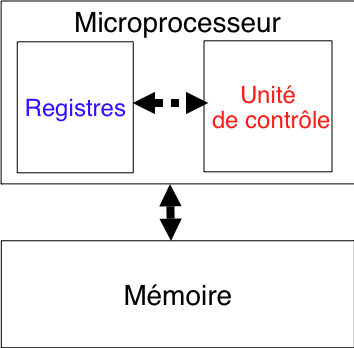
\includegraphics[width=0.3\textwidth]{vanNeumann}
  \caption{\label{fig:vanNeumann}Modèle de von Neumann}
\end{wrapfigure}

Un des premiers principes fondateurs est le modèle d'architecture de \textit{von Neumann}\footnote{Introduit avec le développement des premiers ordinateurs durant la seconde guerre mondiale mais reste tout à fait valide aujourd'hui.} (Figure \ref{fig:vanNeumann}).
La partie la plus intéressante de ce modèle organisé autour de 2 types de dispositifs :
\begin{itemize}
  \item L'unité centrale ou \textbf{\textit{processeur}} qui peut être décomposée en 2 partie :
    \begin{itemize}
      \item L'unité de commande : Permet de charger, décoder et exécuter les instructions du programme qui sont stockées en mémoire.
      \item L'unité arithmétique et logique : Regroupe les circuits électroniques qui permettent d'effectuer les opérations arithmétiques (addition, soustraction, division, ...) et logiques.
        C'est cette unité qui réalise les calculs proprement dits.
    \end{itemize}
  \item La \textbf{\textit{mémoire}} qui joue un double rôle :
    \begin{itemize}
      \item Stocke les données qui sont traitées par le programme;
      \item Stocke les instructions qui composent ce programme.
    \end{itemize}
\end{itemize}

\subsection{La mémoire}
\paragraph{Première approche} En première approximation, on peut considérer la mémoire comme étant un dispositif qui permet de stocker des données binaires.
La mémoire est découpée en blocs de un octet.
Chacun de ces blocs est identifié par une adresse, qui est elle aussi représentée sous la forme d'un nombre binaire.
Une mémoire que permet de stocker $2^k$ bytes de données utilisera au minimum $k$ bits pour représenter l'adresse d'une zone mémoire\footnote{Par exemple, une mémoire pouvant stocker 64 millions de bytes doit utiliser au moins 26 bits d'adresse}.
En pratique, les processeurs des ordinateurs de bureau utilisent 32 ou 64 bits\footnote{D'ancien processeurs utilisaient 16 ou 20 bits d'adresse}.
Ce nombre de bits utilisés pour représenter une adresse en mémoire limite la capacité totale de mémoire adressable par un processeur.
Ainsi, un processeur qui utilise des adresses sur 32 bits n'est pas capable physiquement d'adresser plus de 4 GBytes de mémoire.


\begin{wrapfigure}{r}{0.5\textwidth}
  \vspace{-0.5cm}
  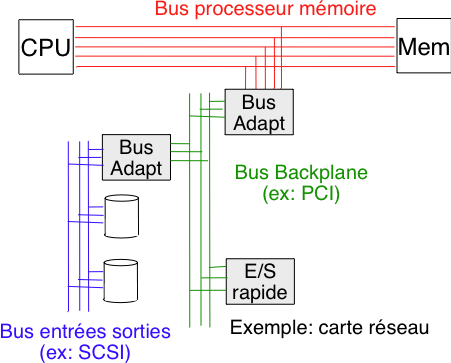
\includegraphics[width=0.5\textwidth]{mem2}
  \caption{\label{fig:vanNeumann}Architecture d'un ordinateur actuel}
\end{wrapfigure}
\paragraph{Approche complexe} En pratique, l'organisation d'un ordinateur actuel est plus complexe que le modèle de von Neumann.
La figure \ref{fig:mem2} présente de manière schématique l'organisation actuelle d'un ordinateur.

Le processeur est directement connecté à la mémoire via un \textbf{\textit{bus}} de communication rapide permettant des échanges de données et d'instructions efficaces entre la mémoire et le processeur.
En plus du proesseur et de la mémoire, un 3e dispositif, souvent appelé \textit{adaptateur de bus} est connecté au bus processeur-mémoire.
Cet adaptateur permet au processeur d'accéder aux dispositifs de stockage ou aux dispositifs d'entrées-sorties tels que le clavier, la souris ou les cartes réseau.
En pratique, cela se réalise en connectant les différents dispositifs à un autre bus de communication (PCI, SCSI,...) et en utilisant un adaptateur de bus qui est capable de traduire les commandes venant du processeur.

\subsubsection*{Mémoires SRAM, DRAM,...}
Les technologies les plus courantes pour la mémoire sont les \textit{SRAM} et les \textit{DRAM}.\\

\noindent\begin{tabularx}{\textwidth}{|l|p{0.32\textwidth}|p{0.25\textwidth}|p{0.25\textwidth}|}
  \hline
  \textbf{Type} & \textbf{Description} & \textbf{Avantages} & \textbf{Inconvénients} \\
  \hline \hline
  \textit{SRAM} & L'information est stockée sous la forme d'un courant électrique qui passe ou ne passe pas à un endroit donné.
  & Temps d'accès assez faible & grande consommation électrique ce qui empêche de développer des mémoires de grandes capacités \\
  \hline
  \textit{DRAM} & C'est la présence ou l'absence d'une charge ($\leq$ à quelques dizaine d'électrons) dans un condensateur qui représente la valeur 0 ou 1.
  & Possible d'en construire de très grande taille : Jusqu'à 1 GByte par chip.
  & Performances nettement moins bonne que les \textit{SRAM}. \\
  \hline
\end{tabularx}
~\\

En pratique, une mémoire \textit{DRAM} actuelle peut être vue comme étant équivalente à une grille.
Les adresse peuvent donc être vues comme étant composée d'un numéro de ligne et d'un numéro de colonne.
Ces deux opérations sont successives.
Lorsque la mémoire a reçu la ligne et ensuite la colonne demandées, avant de pouvoir commencer le transfert de la donnée.
Elles ont donc une latence élevée (par rapport au débit de transfert qui est élevée).
Cela implique que dans une mémoire \textit{DRAM} il est plus rapide de lire ou d'écrire un bloc de 128 bits successifs que quatre blocs de 32 bits à des endroits différents en mémoire.


\subsubsection*{Importance de la mémoire}
Le processeur interagit en permanence avec la mémoire, que ce soit pour charger des données à traiter ou pour charger les instructions\footnote{Certains processeurs utilisent des instructions de taille fixe, par exemple chaque instruction est encodée sous la forme d'un mot de 32 bits.
  D'autres processeurs, comme ceux qui implémentent l'architecture IA32, utilisent des instructions qui sont encodées sous la forme d'un nombre variable de bytes.
Mais cela n'a au final assez peu d'impact sur le développeur de programmes.}.
Les données échangées (données et instructions) sont représentées sous la forme de nombres binaires.
Il est important de prendre conscience de que le processeur doit en permanence charger des données et des instructions depuis la mémoire pour pouvoir exécuter un programme.
Ces échanges peuvent donc avoir un impact sur la vitesse d'exécution comme nous le verrons plus tard

\subsubsection*{Registre}
Outre des unitées de calcul, un processeur contient plusieurs registres.
Un \textit{registre} est une zone de mémoire très rapide se trouvant sur le processeur.
Sur les processeurs courants, cette zone de mémoire permet de stocker un mot de 32 bits ou un long mot de 64 bits.\footnote{Les premiers processeurs disposaient d'un registre unique appelé l'\textit{accumulateur}.
Les processeurs actuels en ont généralement une dizaine ou quelques dizaines.}.
Chaque registre est identifié par un nom ou un numéro et les instructions du processeur permettent d'accéder directement aux données se trouvant dans un registre particulier.
Les registres sont les mémoires les plus rapides qui sont disponibles sur un ordinateur.
Malheureusement, il sont en nombre très limité et il est impossible de faire fonctionner des programmes en utilisant uniquement des registres.

\subsubsection*{Dilemme : Performance VS capacité / prix / faisabilité}
Il serait préférable de pouvoir construire un ordinateur équipé uniquement de SRAM, mais au niveau de la capacité et du prix c'est impossible\footnote{sauf quelques cas rares d'applications spécifiques qui nécessitent de hautes performances et se contentent d'une capacité limitée}.
Les ordinateurs actuels contiennent donc à la fois de la mémoire SRAM et de la mémoire DRAM.
Avec les registres, les SRAM et les DRAM composent les 3 premiers niveaux de la \textit{hiérarchie de la mémoire}.
Il est utile de voir comment cette hiérarchie de mémoire est organisée en pratique en évaluant les différentes alternatives\footnote{En 1980 ce n'était pas vraiment utile car la mémoire était nettement plus rapide que le processeur.
  Mais à partir de 1990 on commence à voir cette tendance s'inverser et les mémoires deviennent un frein par rapport aux processeurs dont les performances se sont fortement améliorés.
Voir slides pour les graphes.}.

\paragraph{1e solution : Répartition d'adresse entre SRAM et DRAM}
Une première solution pour combiner la SRAM et la DRAM serait de réserver par exemple les adresses basses à la SRAM et les adresses hautes à la DRAM.
Avec cette solution, le programme stocké dans la SRAM pourrait s'exécuter nettement plus rapidement que le programme stocké en DRAM.
Il faudrait alors imaginer que l'OS fournissent des appels système permettant aux applications de demander à déplacer certaines parties du programme et des données en SRAM.
Ce genre de solution obligerait chaque application à pouvoir déterminer quelles sont les données et les instructions à exécuter en mémoire SRAM pour obtenir de meilleur performance.
Théoriquement c'est envisageable mais en pratique ça n'a que très peu de chance de fonctionner.


\paragraph{2e solution : La mémoire cache}
Une deuxième solution est d'utiliser le principe de la \textit{\textbf{mémoire cache}}.
Une mémoire cache est une mémoire de faible capacité mais rapide qui est capable de stocker des données provenant de mémoire de plus grande capacité mais plus lente.
Cette mémoire cache sert d'interface entre le processeur et la mémoire principale.
Toutes demandes d'accès à la mémoire principale passent par la mémoire cache comme illustré ci-dessous : \\
\begin{center}
  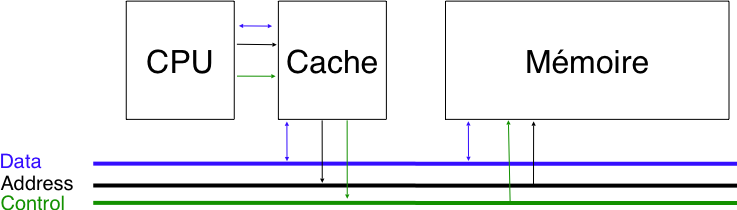
\includegraphics[width=0.5\textwidth]{memcache1}
\end{center}

\subsubsection*{Mémoire cache}

Ce système de mémoire cache est largement utilisé dans les systèmes informatiques afin d'améliorer les performances.
En pratique les mémoires cache utilisent le \textit{\textbf{principe de localité}}.
Il existe deux types de localité :
\begin{itemize}
  \item La \emph{localité temporelle} : Si un processeur accède à la mémoire à l'adresse $A$ à un instant $t$, il est fort probable qu'il y accédera encore dans les instants qui suivent\footnote{Exemple : Lors de l'exécution de boucles qui exécutent à de nombreuses reprises les mêmes instructions}.
  \item La \emph{localité spatiale} : Si un programme a accédé à l'adresse $A$ à l'instant $t$, il est fort probable qu'il accédera aux adresses proches de $A$ comme $A+4$ ou $A-4$ dans les instants qui suivent\footnote{Exemple : Lorsqu'un programme traite un vecteur stocké en mémoire}.
\end{itemize}
\begin{wrapfigure}{r}{0.4\textwidth}
  \vspace{-0.5cm}
  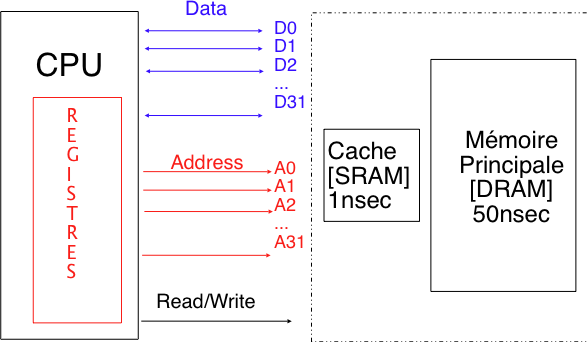
\includegraphics[width=0.45\textwidth]{memhierarchie}
  \caption{\label{fig:memhierarchie}Hiérarchie de la mémoire}
  \vspace{-0.5cm}
\end{wrapfigure}

Les mémoires caches exploitent ces principes de localité en stockant de façon transparente les instructions et les données les plus récemment utilisées.
D'un point de vue physique, on peut voir le processeur comme étant connecté à la (ou les) mémoire(s) cache qui est elle-même connecté à la mémoire \textit{RAM}.\\



Les opérations de lecture en mémoire se déroulent généralement comme suit :
\begin{enumerate}
  \item[1.] Le processeur a besoin de lire une donnée se trouvant a une adresse $A$.
    Il fournit donc cette adresse $A$ à la mémoire cache.
  \item[2a.] Si la donnée correspondante à $A$ est présente en mémoire cache, celle-ci répond directement au processeur.
  \item[2b.] Sinon, la mémoire cache interroge la mémoire \textit{RAM}, se met à jour et ensuite fournit la donnée demandée au processeur.
\end{enumerate}
Ce mode de fonctionnement permet de profiter de la localité temporelle.
Pour profiter de la localité spatiale, la plupart des caches se mettent à jour en chargeant directement une \textit{ligne de cache} qui peut compter jusqu'à quelques dizaines d'adresses en mémoire\footnote{Ce qui permet de profiter des mémoires \textit{DRAM} qui aujourd'hui sont souvent optimisées pour fournir des débits de transfert élevés pour de longs blocs consécutifs en mémoires.}.

\paragraph{Opération d'écriture} Pour les opérations d'écriture, la situation est plus compliquée.
Si le processeur écrit l'information $x$ à l'adresse $A$ en mémoire, il faudrait idéalement que cette valeur soit écrite simultanément en mémoire cache et en mémoire \textit{RAM} de façon à s'assurer que la mémoire \textit{RAM} contient toujours des données à jour.
Pour ce faire, analysons les stratégie :
\begin{itemize}
  \item La stratégie d'écriture la plus simple est baptisée \emph{write through}.
    Avec cette stratégie, toute demande d'écriture venant du processeur donne lieu à une écriture en mémoire cache et une écriture en mémoire \textit{RAM}.
    Cela garantit qu'à tout moment la mémoire cache et la mémoire \textit{RAM} contiennent la même information.
    Malheureusement cette technique n'est pas performante et n'est donc pas acceptable !
  \item L'alternative est d'utiliser la technique du \emph{write back}.
    Avec cette technique, toute écriture est faite en mémoire cache directement.
    Ce qui permet d'obtenir de très bonne performance pour les opérations d'écritures.
    La donnée n'est ré-écrite en mémoire \textit{RAM} que lorsqu'elle doit être retirée de la mémoire cache.
    Cette ré-écriture est faite automatiquement par la mémoire cache.
    Pour la plupart des programmes, la gestion des opérations d'écriture est transparente.
    Il faut cependant être attentif à la technique d'écriture utilisée lorsque plusieurs dispositifs peuvent accéder directement à la mémoire \textit{RAM} sans passer par le processeur\footnote{C'est le cas notamment des cartes réseaux ou de certains contrôleurs de disque dur.
      Pour des raisons de performances, ces dispositifs peuvent copier des données directement de la mémoire \textit{RAM} vers le réseau ou un disque dur.
    Si une écriture de type \emph{write back} est utilisée, le système d'exploitation doit veiller à ce que les données qui ont été écrites par le processeur en cache aient bien été écrites également en mémoire \textit{RAM} avant d'autoriser la carte réseau ou le contrôleur de disque à effectuer un transfert.}.
\end{itemize}

\section{Étude de cas : Architecture IA32}
Cette architecture recouvere un grand nombre de variantes qui ont leur spécificités propre.
L'architecture IA32 est supportée par différents types de processeurs.
Certains utilisent des registres et des bus de données de 32 bits.
D'autres, plus récents utilisent des registres de 64 bits.
Il y a des différences importantes entre ces deux architectures.
Comme les processeurs récents supportent à la fois les modes 32 bits et 64 bits, nous nous limiterons à l'architecture 32 bits ici.


Un élément important d'un processeur tel que ceux de l'architecture IA32 sont ses registres.
Un processeur IA32 dispose de huit registres génériques.
Ceux-ci sont baptisés \texttt{EAX}, \texttt{EBX}, \texttt{ECX}, \texttt{EDX}, \texttt{EBP}, \texttt{ESI}, \texttt{EDI} et \texttt{ESP}.
Ces registres peuvent stocker des données sous forme binaire.
Dans l'architecture IA32, ils ont une taille de 32 bits.
Cela implique que chaque registre peut contenir un nombre ou une adresse puisque les entiers (\texttt{int} en C) et les adresse (pointeurs \texttt{*} en C) sont tous les deux encodés sur 32 bits dans l'architecture IA32.
Cette capacité à stocker des données ou des adresses à l'intérieur d'un même registre est un des points clés de la flexibilité des microprocesseurs.


\texttt{EBP} et \texttt{ESP} sont utilisés dans la gestion de la pile\footnote{Voir aussi la section \ref{manip_de_la_pile} à la page \pageref{manip_de_la_pile}}.
%TODO Comme nous le verrons plus tard...

Tout processeur contient un registre spécial qui stocke à tout moment l'adresse de l'instruction courante en mémoire.
Ce registre est souvent dénommé le \emph{compteur de programme} ou \emph{program counter} (PC).
Dans l'architecture IA32, il s'agit du registre \texttt{EIP} qui stocke l'\emph{Instruction Pointer} qui joue ce rôle.
Ce registre ne peut être utilisé pour effectuer des opérations arithmétiques.
Il peut cependant être modifié par les instructions de saut et joue un rôle essentiel dans l'implémentation des instruction de contrôle.


\begin{wraptable}{r}{0.4\textwidth}
  \begin{tabular}{|c|c|c|}
    \hline
    \multirow{2}*{\textbf{Type}} & \textbf{Taille} & \textbf{Suffixe} \\
                                 & \textbf{(bytes)} & \textbf{assembleur} \\
    \hline \hline
    \texttt{char} & 1 & b \\
    \hline
    \texttt{short} & 2 & w \\
    \hline
    \texttt{int} & 4 & l \\
    \hline
    \texttt{long int} & 4 & l \\
    \hline
    \texttt{void *} & 4 & l \\
    \hline
  \end{tabular}
  \caption{\label{table:ia32types}Types de données supportés par les processeurs IA32}
\end{wraptable}
Outre ces registres génériques, les processeurs de la famille IA32 contiennent aussi des registres spécialisés pour manipuler les nombres en virgule flottante (\texttt{float} et \texttt{double})\footnote{Mais ça c'est hors matière de ce cours}.
Les processeurs IA32 contiennent également des drapeaux regroupés dans le registre \texttt{eflags}.
Ceux-ci sont utilisés pour implémenter différents tests et comparaisons. \\

Les processeurs qui implémentent les spécifications IA32 supportent les types de données repris dans la table \ref{table:ia32types}.
\\

Voyons maintenant les quelques instructions de l'architecture IA32 qui permettent de manipuler des nombres entiers.

\subsection{Les instructions \texttt{mov}}
Les instructions de la famille\footnote{On parle de famille d'instructions car il existe de nombreuses instructions de dpélacement en mémoire.
  Les plus simples sont suffixées par un caractère qui indique le type de données transféré.
Exemple : \texttt{movb} permet le transfert d'un byte tandis que \texttt{movl} permet le transfert d'un mot de 32 bits.} \texttt{mov} permettent de déplacer des données entre registres ou depuis la mémoire vers un registre ou d'un registre vers une zone mémoire.\\
Syntaxe générale :
\begin{lstlisting}[language={[x86masm]Assembler}]
mov src, dest ; deplacement de src vers dest
\end{lstlisting}
Il existe une instruction de la famille \texttt{mov} pour chaque type de donnée pouvant être déplacée : \texttt{movb}, \texttt{movw} et \texttt{movl} qui permettent de déplacer respectivement : 1 byte, un mot de 16 bits, et un mot de 32 bits (voir table \ref{table:ia32types}).
\\

En pratique, il y a plusieurs façons de spécifier chaque argument d'une instruction \texttt{mov}\footnote{Certains auteurs parlent alors de \emph{mode d'adressage} pour représenter ces différents types d'arguments même s'il ne s'agit pas toujours d'adresses.}.
Les différents mode sont :
\begin{itemize}
  \item Le mode \emph{registre} : Pour spécifier que la source et/ou la destination est un registre.
    Le nom du registre est alors préfixé par \texttt{\%}.
  \item Le mode d'adressage \emph{immédiat} : Ne peut être utilisé que pour l'argument source.
    Il permet de placer une constante dans un registre, par exemple pour initialiser sa valeur.
    Il se reconnaît à l'utilisation du symbole \texttt{\$} comme préfixe de la constante.
  \item Le mode d'adressage \emph{absolu} : Dans ce mode, l'un des arguments de l'instruction \texttt{mov} est une adresse en mémoire.
  \item Le mode d'adressage \emph{indirect} : Au lieu de spécifier directement une adresse, on spécifie un registre dont la valeur est une adresse en mémoire ($\approx$ utilisation des pointeurs en langage C).
    Il se reconnaît à l'utilisation des parenthèses autour du nom du registre source ou destination.
  \item Le mode avec une \emph{base} et un \emph{déplacement}.
    Ce mode peut être vu comme une extension du mode indirect.
    Il permet de lire en mémoire à une adresse qui et obtenue en additionnant un entier positif ou négatif, à une adresse stockée dans un registre.
    Ce mode d'adressage joue un rôle important dans le fonctionnement de la pile.
\end{itemize}

\begin{lstlisting}[language={[x86masm]Assembler}, emph={\$,\%,(,),movl},emphstyle={\color{blue}\bfseries}]
; EXEMPLE MODE REGISTRE
movl %eax, %ebx	; deplacement de %eax vers %ebx
movl %ecx, %ecx	; aucun effet

; EXEMPLE MODE IMMEDIAT
movl $0, %eax		; initialisation de %eax a 0
movl $1252, %ecx	; initialisation de %ecx a 1252

; EXEMPLE MODE ABSOLU
movl 0x04, %eax		; place la valeur contenue a l'adresse 0x04 en memoire dans %eax
movl $1252,	%ecx	; initialisation de %ecx a 1252
movl %ecx, 0x08		; remplace le contenu de la memoire a l'adresse 0x08 par 1252

; EXEMPLE MODE INDIRECT
movl $0x08, %eax	; place la valeur 0x08 dans %eax
movl (%eax), %ecx	; place la valeur se trouvant a l'adresse qui est dans
; %eax dans le registre %ecx
movl 0x10, %eax		; place la valeur se trouvant a l'adresse 0x10 dans %eax
movl %ecx, (%eax)	; place le contenu de %ecx a l'adresse qui est contenue
; dans %eax(0x10)

; EXEMPLE MODE AVEC UNE BASE ET UN DEPLACEMENT
movl $0x08,%eax		; place la valeur 0x08 dans %eax
movl 0(%eax), %ecx	; place la valeur se trouvant a l'adresse 0x08 dans le
; registre %ecx
movl 4(%eax), %ecx	; place la valeur se trouvant a l'adresse 0x0C (=0x08+4) dans
; le registre %ecx
movl -8(%eax), %ecx	; place la valeur se trouvant a l'adresse 0x00 (=0x08-8) dans
; le registre %ecx
\end{lstlisting}
%$
L'architecture IA32 supporte encore d'autres modes d'adressage (non vu dans le cours).
Une autre instruction permettant de déplacer de l'information est l'instruction \texttt{leal} (load effective address).
Cette instruction place dans le registre destination l'adresse de son argument source plutot que sa valeur.
Par exemple : \texttt{leal 4(\%esp) \%edx} placera dans le registre \texttt{\%edx} l'adresse de son argument source, c'est-à-dire l'adresse contenue dans \texttt{\%esp+4}.

\subsection{Les instructions arithmétiques et logiques}
La 2e famille d'instructions importante sur un processeur sont les instructions qui permettent d'effectuer les opérations arithmétiques et logiques.
Les instructions les plus simples sont celle qui prennent un seul argument :
\begin{itemize}
  \item \texttt{inc} : incrémente d'une unité la valeur stockée dans le registre/l'adresse fournie en argument et sauvegarde le résultat de l'incrémentation au même endroit.
    Cette instruction peut être utilisée pour implémenter des compteurs de boucles.
  \item \texttt{dec} : même principe que \texttt{inc} mais pour décrémenter.
  \item \texttt{not} : applique l'opération logique \texttt{NOT} à son argument et stocke le résultat au même endroit.
\end{itemize}
De même que pour \texttt{mov}, il existe une variante de chaque instruction ci-dessus pour chaque type de données : \texttt{incb}, \texttt{incw}, \texttt{incl},...
(voir de nouveau la table \ref{table:ia32types}).\\

L'architecture IA32 supporte également des instructions arithmétiques et logiques prenant deux arguments :
\begin{itemize}
  \item \texttt{add} : Permet d'additionner deux nombres entiers.
    Prend comme arguments une source et une destination et place dans la destination la somme de ses deux arguments.
  \item \texttt{sub} : Permet de soustraire le premier argument du second.
    Stocke le résultat dans le second.
  \item \texttt{mul} : Permet de multiplier des nombres entiers non-signés.
    (\texttt{imul} permet la multiplication de nombres signés)
  \item \texttt{div} : Permet la division de nombres entiers non-signés.
  \item \texttt{shl} (reps. \texttt{shr} : Permet de réaliser un décalage logique vers la gauche (resp. droite).
  \item \texttt{xor} : Calcul le ou exclusif entre ses deux arguments et sauvegarde le résultat dans le second.
  \item \texttt{and} : Calcul la conjonction logique entre ses deux arguments et sauvegarde le résultat dans le second.
\end{itemize}


\subsection{Les instructions de comparaison}
Les comparaisons sont nécessaires pour implémenter des tests tels que \texttt{if (condition) \{ ... \} else \{ ... \}}.
Sur les processeurs IA32, les comparaisons utilisent des drapeaux qui sont mis à jour par le processeur après l'exécution de certaines instructions.
Ceux-ci sont regroupés dans le registre \texttt{eflags}.
Les principaux drapeaux sont :
\begin{itemize}
  \item \emph{ZF} (Zero Flag) : Indique si le résultat de la dernière opération était zéro
  \item \emph{SF} (Sign Flag) : Indique si le résultat de la dernière instruction était négatif.
  \item \emph{CF} (Carry Flag) : Indique si le résultat de la dernière instruction arithmétique non signée nécessitait plus de 32 bits pour être stocké.
  \item \emph{OF} (Overflow Flag) : Indique si le résultat de la dernière instruction arithmétique signée a provoqué un dépassement de capacité.
\end{itemize}

Nous utiliserons principalement les drapeaux \textit{ZF} et \textit{SF} dans ce "chapitre".
Ces drapeaux peuvent être fixés par les instructions arithmétiques standard, mais aussi par
\begin{itemize}
  \item \texttt{cmp} : Effectue l'équivalent d'une soustraction et met à jour les drapeaux \textit{CF} et \textit{SF} mais sans sauvegarder son résultat dans un registre.
  \item \texttt{test} : Effectue une conjonction logique en mettant à jour les drapeaux mais sans sauvegarder son résultat.
\end{itemize}

Ces instructions de comparaison peuvent être utilisées avec les instructions \texttt{set} qui permettent de fixer la valeur d'un registre en fonction des valeurs de certains drapeaux du registre \texttt{eflags}.
Chaque instruction \texttt{set} prend comme argument un registre.
Pour des raisons historiques, ces instructions modifient uniquement les bits de poids faible du registre indiqué et non le registre complet.
\begin{itemize}
  \item \texttt{sete} : Met le registre argument à la valeur du drapeau \textit{ZF}.
    Permet d'implémenter une égalité
  \item \texttt{sets} : Met le registre argument à la valeur du drapeau \textit{SF}.
  \item \texttt{setg} : Place dans le registre argument la valeur \texttt{\~{}SF \& \~{}ZF} (tout en prenant compte les dépassements éventuels avec \texttt{OF}).
    Permet d'implémenter la condition \texttt{>}.
  \item \texttt{setl} : Place dans le registre argument la valeur \texttt{SF} (tout en prenant compte les dépassements éventuels avec \texttt{OF}).
    Permet d'implémenter la condition \texttt{<=}.
\end{itemize}

\subsection{Les instructions sauts}
Les instructions de saut sont des instructions de base pour tous les processeurs.
Elles permettent de modifier la valeur du compteur de programme \texttt{\%epi} de façon à modifier l'ordre d'exécution des instructions.
Elles sont nécessaires pour implémenter les tests, les boucles et les appels de fonction.
Les premiers langages de programmation et les langages tels que le BASIC ou FORTRAN disposent d'une construction similaire avec l'instruction \texttt{goto}.
Cependant, l'utilisation de l'instruction \texttt{goto} dans des programmes de haut niveau rend souvent le code difficile à lire et de nombreux langages de programmation n'ont plus de \texttt{goto}\footnote{Le C permet encore l'utilisation de \texttt{goto} (contrairement à Java) mais son utilisation est fortement déconseillée !}.
Lors de l'exécution d'un \texttt{goto}, le programme saute directement à l'exécution de l'instruction qui suit le label indiqué.



En assembleur, les instructions de saut sont inévitables.
L'instruction de saut la plus simple est \texttt{jmp}.
Elle prend généralement comme argument une étiquette.
Dans ce cas, l'exécution du programme après l'instruction \texttt{jmp} se poursuivra par l'exécution de l'instruction qui se trouve à l'adresse correspondant à l'étiquette fournie en argument.
Il est également possible d'utiliser l'instruction \texttt{jmp} avec un registre comme argument.
Ainsi, l'instruction \texttt{jmp *\%eax} indique que l'exécution du programme doit se poursuivre par l'exécution de l'instruction se trouvant à l'adresse qui est contenue dans le registre \texttt{\%eax}.\\

Il existe plusieurs variantes conditionnelles de l'instruction \texttt{jmp}.
Ces variantes sont exécutées uniquement si la condition correspondante est vérifiée; les plus fréquentes sont :
\begin{itemize}
  \item \texttt{je} : saut si égal (teste \textit{ZF}).
  \item \texttt{jne} : inverse de \texttt{je}.
  \item \texttt{js} : saut si négatif (teste \textit{SF})
  \item \texttt{jns} : inverse de \texttt{js}.
  \item \texttt{jg} : saut si strictement supérieur (teste \textit{SF} et \textit{ZF} et prend en compte un overflow éventuel)
  \item \texttt{jl} : inverse de \texttt{jg} (strictement inférieur)
  \item \texttt{jge} : saut si supérieur ou égal (teste \textit{SF} et prend en compte un overflow éventuel)
  \item \texttt{jle} : inverse de \textbf{jge}.
\end{itemize}
Ces variantes sont utilisées pour implémenter des expressions \texttt{if(condition)\{ ...
\} else \{ ...\}} en C ou pour implémenter des boucle \texttt{while} par exemple.

\subsection{Manipulation de la pile}
\label{manip_de_la_pile}
Les instructions \texttt{mov} permettent de déplacer de l'information à n'importe quel endroit de la mémoire.
À côté de ces instructions de déplacement, il y a des instructions qui sont spécialisées dans la manipulation de la pile.
La pile, qui dans un processus Unix est stockée dans les adresses hautes est essentielle au bon fonctionnement des programmes.
Par convention dans l'architecture IA32, l'adresse du sommet de la pile est toujours stockée dans le registre \texttt{\%esp}.

\begin{itemize}
  \item \texttt{pushl \%reg} : Place le contenu du registre \texttt{\%reg} au sommet de la pile et décrémente dans le registre \texttt{\%esp} l'adresse du sommet de la pile de 4 unités.
  \item \texttt{popl \%reg} : Retire le mot de 32 bits se trouvant au sommet de la pile, le sauvegarde dans le registre \texttt{\%reg} et incrémente dans le registre \texttt{\%reg} l'adresse du sommet de la pile de 4 unités.
\end{itemize}
(En pratique ces instructions de manipulation de pile pourraient être écrite un utilisant \texttt{subl}, \texttt{movl} et \texttt{addl}, voir p74).

\subsection{Les fonctions et procédures}
Les fonctions et les procédures sont essentielles dans tout langage de programmation.
Une procédure est une fonction qui ne retourne pas de résultat.

Une procédure est un ensemble d'instructions qui peuvent être appelées depuis n'importe quel endroit du programme.
Généralement, une procédure est appelée depuis plusieurs endroits différents d'un programme.
Considérons d'abord une procédure en C ne prenant aucun argument (\texttt{void uneProcedure()}) : \\
Le processeur doit transférer l'exécution du code à la première instruction de la procédure appelée.
Cela se fait en associant une étiquette à chaque procédure qui correspond à l'adresse de la première instruction de cette procédure.
Il est également nécessaire que la procédure puisse connaître l'adresse de l'instruction qui doit être exécutée à la fin de son exécution.
Dans l'architecture IA32, cela se fait en utilisant la pile.
Vu l'importance des appels de procédure et de fonctions, l'architecture IA32 contient 2 instructions dédicacées pour implémenter ces appels.
\begin{itemize}
  \item \texttt{call} : Instruction de saut qui transfère l'exécution à l'adresse de l'étiquette passée en argument et en plus elle sauvegarde au sommet de la pile l'adresse de l'instruction qui la suit.
    Elle est équivalent à une instruction \texttt{push} suivit d'une instruction \texttt{jmp}.
  \item \texttt{ret} : Instruction de saut qui suppose que l'adresse de retour se trouve au sommet de la pile, retire cette adresse de la pile et fait un saut à cette adresse.
    Elle est équivalent à une instruction \texttt{pop} suivit d'une instruction \texttt{jmp}.
    Dans l'architecture IA32, le registre \texttt{\%esp} contient en permanence le sommet de la pile, il est donc utilisé par \texttt{call} et \texttt{ret}.
\end{itemize}
%TODO : Il y a une convention de l'architecture IA32 qui veut que les adresses de retour des procédures soient allignées sur des blocs de 16 bytes (voir page 76).

Considérons maintenant une procédure qui prend un argument.
Pour qu'une telle procédure puisse utiliser son argument,
il faut que la procédure appelante puisse placer sa valeur à un endroit où la procédure appelée peut facilement y accéder.
Dans l'architecture IA32, c'est la pile qui joue ce rôle et permet le passage des arguments.
En C, les arguments sont passés par valeur et ce sera donc la valeur des arguments qui sera placée sur la pile.
La fonction appelante sauvegarde également d'autres registres sur la pile avant l'appel de la fonction.
Ces sauvegardes sont nécessaires car la fonction appelante ne sait pas quels registres seront modifiés par la fonction qu'elle appelle.
Par convention, dans l'architecture IA32, ce sont les registres \texttt{\%eax}, \texttt{\%edx} et \texttt{\%ecx} qui sont sous la responsabilité de la procédure appelante.
Une procédure appelée peut modifier sans limite les valeurs de ces registres.
D'autre part les registres \texttt{\%ebx}, \texttt{\%edi} et \texttt{\%esi} sont sous la responsabilité de la procédure appelée et doivent être sauvé par celle-ci si elle désire les utiliser/modifier.


Une fonction - contrairement aux procédure - retourne un résultat.
Pour ce faire il faut que la procédure appelante puisse savoir où aller
chercher ce résultat après l'exécution de l'instruction \texttt{ret}.
La valeur de retour d'une fonction est stockée par convention
dans le registre \texttt{\%eax}.\\

En vue du fonctionnement des appels de fonction en assembleur, on comprend aisément que l'utilisation de fonctions récursives en C à un coût important au niveau de la gestion de la pile.
Ces appels récursifs doivent donc être réservés à des fonctions où l'appel récursif apporte une plus value claire et ne peux pas être réalisé par une fonction itérative.

\section{Les threads}
(Voir évolution des performances des processeurs dans le cours page 95-98)

La notion de thread d'exécution est très importante
dans un système informatique.
Elle permet de comprendre comment un ordinateur équipé d'un seul microprocesseur peut exécuter plusieurs programme simultanément mais aussi comment des programmes peuvent profiter des nouveaux processeurs (\emph{multi-cœurs} ou \emph{multi-threadé}) capables d'exécuter plusieurs threads simultanément.

Pour rappel, pour qu'un processeur puisse exécuter une séquence d'instruction,
il faut non seulement qu'il implémente chaque instruction
mais également qu'il puisse accéder :
\begin{itemize}
  \item à la mémoire contenant les instructions à exécuter
  \item à la mémoire contenant les données manipulées
    par cette séquence d'instruction : C'est-à-dire
    \begin{itemize}
      \item la zone contenant les variables globales
      \item le tas
      \item la pile
    \end{itemize}
  \item aux registres, et plus particulièrement :
    \begin{itemize}
      \item aux registres de données pour stocker les résultats de chacune des instructions.
      \item au registre \texttt{\%esp} directement ou indirectement via les instructions \texttt{push} et \texttt{pop} de manipulation de la pile
      \item au registre \texttt{\%eix} qui contient l'adresse de l'instruction en cours d'exécution
      \item au registre \texttt{eflags} qui contient l'ensemble des drapeaux.
    \end{itemize}
\end{itemize}

Un processeur multithreadé a la capacité d'exécuter plusieurs programmes simultanément, pour ce faire il disposera de copies des registres.
Chacun de ces bloc de registres pourra être utilisé pour exécuter ces programmes simultanément à raison d'un thread d'exécution par bloc de registres.
Chaque thread d'exécution va correspondre à une séquence différente d'instructions qui va modifier son propre bloc de registres.\\
Cette capacité d'exécuter plusieurs threads d'exécution simultanément n'est pas limitée à un thread d'exécution par programme puisqu'au final, un thread d'exécution n'est finalement qu'une séquence d'instructions qui utilisent un bloc de registres.
En pratique pour qu'un programme puisse démarrer un nouveau thread d'exécution sur un nouveau bloc de registre, cela nécessite la coopération avec l'OS.
Le mécanisme le plus courant pour ce faire est connu sous le nom de \emph{threads POSIX}.



\subsection{Les threads POSIX}
Les threads POSIX sont supportés par la plupart des variantes Unix et sont souvent implémentés dans une librairie (\texttt{pthreads} sous linux).
Les fonctions importantes de cette librairie sont :
\begin{itemize}
  \item \texttt{\textbf{int} pthread\_create(pthread\_t *\textbf{restrict thread}, \textbf{const} pthread\_attr\_t *\textbf{restrict} attr, \textbf{void} *(*start\_routine)(\textbf{void} *), \textbf{void} *\textbf{restrict} arg);}\\
    Permet de créer un nouveau thread d'exécution\footnote{Il est important de veiller à ce que le quatrième argument passé à \texttt{pthread\_create} existe toujours (et n'ait pas été modifiée) au moment de l'exécution effective de la fonction qui démarre le thread lancé.
    }.
  \item \texttt{\textbf{int} pthread\_join(pthread\_t \textbf{thread}, \textbf{void} **value\_ptr);}\\
    Permet de récupérer le résultat d'un thread d'exécution.
    L'appel de \texttt{pthread\_join} ne se terminera que lorsque le thread spécifié se terminera.
  \item \texttt{\textbf{void} pthread\_exit(\textbf{void} *retval);}\\
    Le thread qui exécute cette fonction se termine et retourne la valeur \texttt{retval} au thread parent.
    (Également possible avec un \texttt{return})
  \item \texttt{\textbf{int} pthread\_attr\_setstackaddr(pthread\_attr\_t *attr, \textbf{void} *stackaddr); }\\
    Permet de modifier la taille de la pile d'un thread POSIX (Utile si on sait qu'un thread devra allouer un grand tableau auquel il sera le seul à avoir accès).
\end{itemize}

\subsubsection{Variables \texttt{volatile}}
Normalement, dans un programme C, lorsqu'une variable est définie, ses accès sont contrôlés entièrement par le compilateur.
Si une variable est utilisée dans plusieurs calculs successifs, afin d'obtenir de bonne performance, il peut être utile de stocker sa valeur dans un registre durant le temps des calculs.
Mais dans le cas où cette valeur pourrait être modifié par d'autres threads simultanément il peut être utile d'indiquer qu'il faut recharger sa valeur avant chaque calcul, cela se fait en utilisant le qualificatif \texttt{volatile} qui indique au compilateur qu'il doit recharger la variable de la mémoire chaque fois qu'elle est utilisée.
(à utiliser avec précaution, voir partie sur les mutex etc.)

\subsubsection{Variable spécifique à un thread}
Pour ce faire, il existe 2 solutions :
\begin{itemize}
  \item Utiliser le qualificatif \texttt{\_\_thread} devant une déclaration de variable (supporté par gcc avec la librairie threads POSIX).
  \item Utiliser les fonctions fournies par la librairie threads POSIX suivantes : \texttt{pthread\_key\_create}, \texttt{pthread\_key\_set}, \texttt{pthread\_setspecific}, \texttt{pthread\_getspecific} et \texttt{pthread\_key\_delete}.
\end{itemize}
La deuxième solution est plus compliquée à utilisée mais illustre ce qu'il se passe en pratique lorsque le qualificatif \texttt{\_\_thread} est utilisé.

\subsection{Fonctions thread-safe}
Certaines fonctions (même de la librairie standard) sont susceptible d'utiliser des variables globales dans leur exécution, et utilisent l'hypothèse qu'elles sont appelées par un programme séquentiel ce qui peut poser des problèmes.
Lorsque l'on développe une fonction qui peut être réutilisée, il est important de s'assurer que cette fonction peut être exécutée par plusieurs threads simultanément sans que cela ne pose de problèmes à l'exécution.
C'est pourquoi lorsque l'on intègre des fonctions provenant de la librairie standard ou d'une autre librairie dans un programme découpé en threads, il est important de vérifier que les fonctions utilisées sont bien \textbf{\textit{thread-safe}}.
La page de manuel \texttt{man 7 pthreads} liste les fonctions qui ne le sont pas.



\section{Threads communicants}
Lorsqu'un programme est décomposé en plusieurs threads, ceux-ci doivent en général communiquer entre eux.

\begin{wrapfigure}{r}{0.4\textwidth}
  \vspace{-0.5cm}
  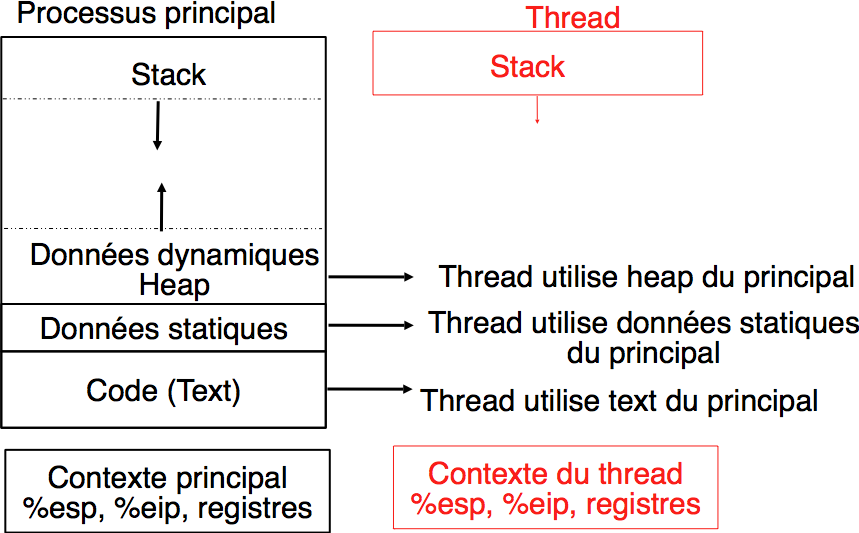
\includegraphics[width=0.5\textwidth]{memthread}
  \caption{\label{fig:memthread}Organisation de la mémoire après la création d'un thread POSIX}
  \vspace{-0.7cm}
\end{wrapfigure}
Le programme principal et le thread qu'il a créé partagent 3 zones de mémoires :
\begin{itemize}
  \item le \emph{segment text} (contient l'ensemble des instructions)
  \item le \emph{segment de données} (contient toutes les données statiques, initialisées ou non)
  \item le \emph{heap}
\end{itemize}
Par contre, le programme principal et le thread qu'il vient de créer ont chacun leur propre contexte et leur propre pile.

\subsection{Loi de Amdahl}
Gene Amdahl considère qu'un programme $P$ peut être découpé en deux partie :
\begin{itemize}
  \item Une partie purement séquentielle.
    Il s'agit par exemple de l'initialisation de l'algorithme utilisé, de la collecte des résultats,...
  \item une partie qui est parallélisable.
    Il s'agit en général du cœur de l'algorithme.
\end{itemize}
Plus les opérations réalisées à l'intérieur d'un programme sont indépendantes entre elles, plus le programme est parallélisable et inversement.\\
Pour Amdahl, si le temps d'exécution d'un programme séquentiel est $T$ et qu'une fraction $f$ de ce programme est parallélisable, alors le gain qui peut être obtenu de la parallélisation en $N$ threads est :
$$\frac{T}{T.((1-f) + \frac{f}{N}} = \frac{1}{(1-f) + \frac{f}{N}} ~~~~~ \text{(loi de Amdahl)}$$
Cette loi fixe une limite théorique difficile à atteindre et suppose que la parallélisation est parfaite c'est à dire que la création et la terminaison des threads n'ont aucun coût en performance.
%\begin{wrapfigure}{r}{0.4\textwidth}
%\vspace{-0.7cm}
%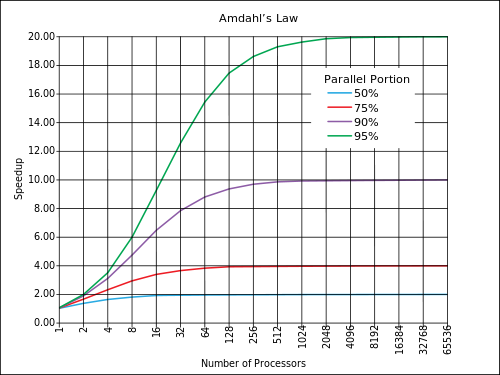
\includegraphics[width=0.5\textwidth]{amdahl}
%\caption{\label{fig:amdahl}Illustration de la loi d'Amdahl}
%\vspace{-0.7cm}
%\end{wrapfigure}
\subsection{Communication entre threads}
Le première façon pour un processus de communiquer des infos avec un thread qu'il a lancé est d'utiliser les arguments de la fonction de démarrage du thread et la valeur retournée par ce thread.
Mais c'est un canal de communication très limité qui ne permet pas d'échange d'information pendant l'exécution du thread.

Un processus peut partager facilement de l'information avec ses threads ou même entre plusieurs threads car tout les threads ont accès aux mêmes variables globales et au même heap.
Malheureusement la modification d'une variable globale ou d'une zone mémoire (allouée par malloc) peut être source de problèmes si plusieurs threads accède à la même donnée en même temps.\\
Ce problème d'accès à une même donnée est connu sous le nom de problème de la \emph{section critique} ou \emph{exclusion mutuelle}.
La \emph{section critique} peut être définie comme étant une séquence d'instructions qui ne peuvent jamais être exécutées par plusieurs threads simultanément.
En pratique on retrouvera une section critique chaque fois que deux threads peuvent modifier ou lire la valeur d'une même zone de la mémoire.
Afin d'éviter ce problème il faut utiliser la coordination entre threads.

\subsection{Coordination entre threads}
\subsubsection{Exclusion mutuelle - Dijkstra}
Le problème de l'exclusion mutuelle à été initialement proposé par Dijkstra (en 1965).
Il peut être reformulé de la façon suivante pour un programme décomposé en threads : \\
Considérons un programme à $N$ threads.
Chaque threads est exécuté cycliquement et possède une section critique et une section non-critique.
La durée d'exécution de chaque partie n'est pas connue et peut être différentes pour chaque thread.
Le problème de l'exclusion mutuelle consiste à trouver un algorithme qui permet de garantir qu'il n'y aura jamais deux threads qui simultanément exécuteront les instructions de leur section critique.\\
\\
Cela revient à dire qu'il n'y aura pas de violation de la section critique.
Cette propriété est une propriété de \textbf{\textit{sureté}} (\textit{safety}).
Dans un programme découpé en threads, une propriété de \textit{sureté} est une propriété qui doit être vérifie à tout instant de l'exécution du programme.

\paragraph{Conditions à satisfaire pour résoudre le problème de l'exclusion mutuelle}
\begin{enumerate}
  \item Tout les threads doivent être considéré de la même façon, on ne peut faire aucune hypothèse sur la priorité relative des différents threads.
  \item On ne peut faire aucune hypothèse sur la vitesse relative ou absolue d'exécution des différents threads.
  \item Doit permettre à un thread de s'arrêter en dehors de sa section critique sans que cela n'invalide la contrainte d'exclusion mutuelle.
  \item Aucun thread qui souhaite entamer sa section critique ne doit être empêché indéfiniment d'y accéder.
\end{enumerate}

La 4e contraintes est un exemple de propriété de \textit{\textbf{vivacité}} (\textit{liveness}).
Une propriété de \textit{vivacité} est une propriété qui ne peut pas être éternellement invalidée.

\subsubsection*{Exclusion mutuelle sur monoprocesseurs}
Sur un ordinateur monoprocesseur, un OS multitâche tel que Unix exécute régulièrement des changement de contexte entre threads.
Le \textit{\textbf{contexte}} d'un thread est composé de l'ensemble des contenus des registres qui sont nécessaires à son exécution (y compris le contenu des registres spéciaux tels que \texttt{\%esp}, \texttt{\%eip} et \texttt{\%eflags}).
Ces registres définissnt l'état du thread du point de vue du processeur. \\
Pour passer d'un thread $T1$ à un thread $T2$ l'OS doit initier un \textbf{\textit{changement de contexte}}.
Pour ce faire il copie le contenu des registres utilisés par $T1$ vers une zone mémoire lui appartenant puis transfère depuis une autre zone mémoire lui appartenant le contexte de $T2$.\\

Sur un système Unix, il y a 2 types d'événements qui peuvent provoquer un changement de contexte.
\begin{itemize}
  \item Le hardware génère une \textit{interruption}.
  \item Un thread exécute un \textit{appel système bloquant}.
\end{itemize}

\paragraph{Interruption : } Une interruption est un signal électronique qui est généré par un dispositifs connectés au microprocesseur. De nombreux dispositifs d'entrées-sorties comme les cartes réseau ou les contrôleurs de disque peuvent générer une interruption lorsqu'une information a été lue ou reçue et doit être traitée par le processeur.
En outre, chaque ordinateur dispose d'une horloge temps réel qui génère des interruptions à une fréquence déterminée par l'OS (entre quelques dizaines et quelques milliers de Hz).
Ces interruptions nécessitent un traitement rapide de la part de l'OS : C'est pourquoi le processeur vérifie, à la fin de l'exécution de \textit{chaque} instruction si un signal d'interruption est présent\footnote{Le cours se limite à un seul type de signa d'interruption}.Si c'est le cas, le processeur sauvegarde en mémoire le contexte du thread en cours d'exécution et lance une routine de traitement d'interruption faisant partie du système d'exploitation.

\paragraph{Appel système :} Un thread exécute un appel système chaque fois qu'il doit intéragir avec l'OS.
Ces appels peuvent être exécutés directement ou via une fonction de la librairie\footnote{La section \texttt{2} du manuel décrits les appels systèmes, la section \texttt{3} décrit les fonctions de la librairie.}.

\begin{itemize}
  \item \textbf{Appel système non-bloquant} est un appel système que l'OS peut exécuter immédiatement.
    Ce type d'appel retourne en général une valeur qui fait partie de l'OS lui-même (par exemple \texttt{gettimeofday}).
  \item \textbf{Appel système bloquant} est un appel système dont le résultat ne peut pas toujours être fourni immédiatement (par exemple : lecture d'information en provenance de l'entrée standard).
    Dans ce cas le thread est mis en attente et aucune instruction de ce thread n'est exécuté tant que le résultat n'est pas connu.
    Le contexte du thread est mis en attente dans une zone mémoire gérée par l'OS.
    Il sera redémarré automatiquement lorsque la donnée attendue sera disponible.
\end{itemize}

La figure \ref{fig:appelsbloquant} représente les différents état d'un thread.
Lorsqu'un thread est crée (avec \texttt{pthread\_create}), il est placé dans l'état \textit{Ready}. \\
\begin{wrapfigure}{r}{0.45\textwidth}
  \vspace{-0.5cm}
  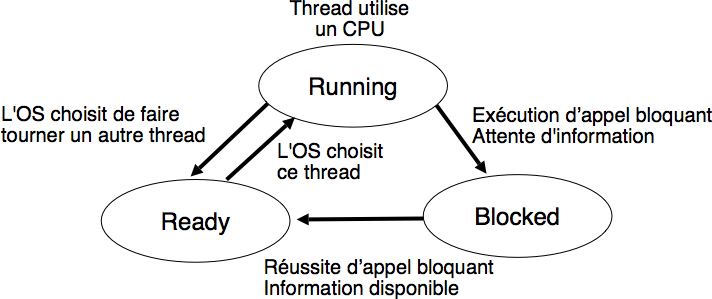
\includegraphics[width=0.55\textwidth]{appelsbloquant}
  \caption{\label{fig:appelsbloquant}États d'un thread d'exécution}
  \vspace{-0.5cm}
\end{wrapfigure}

Les transitions entre les différents états d'un thread sont gérées par l'OS.
Lorsque plusieurs threads d'exécution sont simultanément actifs, l'OS doit arbitrer les demandes d'utilisation du CPU de chaque thread.
Cet arbitrage est réalisé par l'\textit{\textbf{ordonnanceur}} (ou \textbf{\textit{scheduler}}).


\paragraph{Le \textit{scheduler}} est un ensemble d'algorithmes qui sont utilisés par l'OS pour sélectionner le ou les threads qui peuvent utiliser un processeur à un moment donné.
Citons quelques principes de base de fonctionnement de quelques schedulers:
\begin{itemize}
  \item \textbf{le scheduler \textbf{round-robin}} : Ce scheduler maintient en permanence une liste circulaire de l'ensemble des threads qui se trouvent dans l'état \textit{Ready} et un pointeur vers l'élément courant de cette liste.
    En général ce type de scheduler limite le temps passé sur un processeur afin d'éviter qu'un thread ne le monopolise.
    Un scheduler \textit{round-robin} est équitable, si $N$ thread sont actifs en permanence, ils recevront chacun $\frac{1}{N}$ de temps CPU disponible.
  \item \textbf{le scheduler à priorités} : Une priorité est associée à chaque thread.
    Lorsque le scheduler doit sélectionner un thread à exécuter, il commence d'abord par parcourir les threads ayant une haute priorité.
    En pratique le scheduler maintient une liste circulaire par niveau de priorité et s'il y a plusieurs thread pour un niveau de priorité, il utilisera le principe du \textit{round-robin} pour le niveau en question.
\end{itemize}
Sous Unix, il s'agit d'un scheduler à priorité avec un round-robin à chaque niveau de priorité, mais la priorité varie dynamiquement en fonction du temps et des opérations d'entrées sorties effectuées de façon à favoriser les threads interactifs.

Note : Il est possible à un thread d'indiquer explicitement  qu'il peut être remplacé par un autre thread en utilisant \texttt{pthread\_yield} (par exemple utile si on a un thread qui calcul des statistique et ne doit pas ralentir le fonctionnement des autres threads).

\paragraph{Problème de l'exclusion mutuelle, le retour !} Sur une machine monoprocesseur une violation de la section critique ne serait possible qui s'il y a une interruption lorsqu'on est dans celle-ci.
Une solution pour résoudre le problème serait donc de désactiver les interruptions avant la section critique puis de les réactiver après la fin de celle-ci.
Ce serait possible mais
\begin{itemize}
  \item Ça perturbe le fonctionnement de l'OS : sans interruptions, la plupart des opérations d'entrées-sorties et l'horloge sont inutilisable.
    (Donc cette désactivation doit être très courte)
  \item Il s'agit d'une opération privilégiée sur un microprocesseur, il faudrait donc imaginer un appel système qui permettrait à un thread de faire la demande auprès de l'OS.
  \item Si un thread désactiverait les interruptions sans les réactivées après quelques instants, cela rendrait la machine complètement inutilisable puisque sans interruption plus aucune opération d'entrée-sortie n'est possible.
\end{itemize}
Conclusion : Ce n'est pas un mécanisme utilisable\footnote{Bien que ce soit parfois utilisé par certains OS qui l'utilisent à l'intérieur de l'OS même.} !

\subsubsection*{L'algorithme de Peterson}
Cette solution permet à plusieurs threads de coordonner leur exécution de façon à éviter une violation de section critique en utilisant uniquement des variables accessibles à tous les threads.
La solution est applicable à $N$ thread mais nous nous limiterons à 2 threads.

\begin{lstlisting}
#define A 0
#define B 1
int flag[];
flag[A]=false;
flag[B]=false;
// thread A
void* threadA(void* ){
  flag[A]=true;
  turn=B;
  while((flag[B]==true)&&(turn==B)) { /* loop */ }
  section_critique();
  flag[A]=false;
  // ...
}
// Thread B
void* threadB(void* ){
  flag[B]=true;
  turn=A;
  while((flag[A]==true)&&(turn==A))
  { /* loop */ }
  section_critique();
  flag[B]=false;
  // ...
}
\end{lstlisting}

Pour arriver à cet algorithme, les pages 114 à 117 du cours explique les différents raisonnements et problèmes qui y sont liés.
Il faut être attentif au \textit{livelock} et aux conditions énoncées précédemment pour résoudre l'exclusion mutuelle.
Un \textit{livelock} est une situation dans laquelle plusieurs threads exécutent une séquence d'instructions (par exemple une boucle while) sans qu'aucun thread ne puisse réaliser de progrès.
Un \textit{livelock} est un problème gênant puisque lorsqu'il survient les threads concernés continuent à utiliser le processeur mais n'exécutent aucune instruction utile. \\

\subsubsection*{Utilisation d'instruction atomique}
Sur les ordinateurs actuels, il est difficile d'utiliser l'algorithme de Peterson tel que décrit plus haut car
\begin{itemize}
  \item Les compilateurs optimise le code et peuvent supprimer les instructions qui peuvent sembler inutiles.
  \item Sur un ordinateur multi-processeur, chaque processeur peut réordonner les accès à la mémoire automatiquement afin d'en optimiser les performances.
    (Et donc la lecture et l'écriture en mémoire ne se fait pas toujours dans le même ordre que celui prévu initialement)
\end{itemize}
Pour résoudre ce problème, les architectes de microprocesseurs ont proposé l'utilisation d'opérations atomiques.
Une \textbf{opération atomique} est une opération qui lorsqu'elle est exécutée sur un processeur ne peut pas être interrompue par l'arrivée d'une interruption.
De plus, l'exécution d'une instruction atomique par un ou plusieurs processeur implique une coordination des processeurs pour l'accès à la zone mémoire référencée dans l'instruction.
Via un mécanisme qui sort du cadre de ce cours, tous les accès à la mémoire faits par les instruction atomique sont réalisés séquentiellement. \\
\\
Considérons l'instruction \texttt{xchg} supportée par les processeur IA32.
Cette instruction permet d'échanger, de façon atomique, le contenu d'un registre avec une zone de la mémoire.
Elle prend deux arguments : un registre et une adresse en mémoire.
Elle est équivalente à trois instruction \texttt{mov} successive. \\
Avec cette instruction atomique, il est possible de résoudre le problème de l'exclusion mutuelle en  utilisant une zone mémoire (\texttt{lock}) qui prend la valeur \texttt{1} ou \texttt{0}.
Lorsqu'un thread veux exécuter sa section critique, il place la valeur \texttt{1} dans un de ses registre, échange ce registre avec la zone mémoire \texttt{lock} en utilisant \texttt{xchg}.
Si la valeur de son registre en 0, c'est qu'il peut rentrer dans sa section critique, sinon c'est qu'un autre thread est dans sa section critique.
Pour quitter la section critique il suffit ensuite de placer la valeur \texttt{0} en utilisant de nouveau \texttt{xchg}.
Le code ci-dessous montre un exemple :
\begin{lstlisting}[language={[x86masm]Assembler}, emph={\$,\%,(,),movl},emphstyle={\color{blue}\bfseries}]
lock:                    ; etiquette, variable
.long   0          ; initialisee a 0

enter:
movl    $1, %eax      ; %eax=1
xchgl   %eax, (lock)  ; instruction atomique, echange (lock) et %eax
; apres execution, %eax contient la donnee qui etait
; dans lock et lock la valeur 1
testl   %eax, %eax    ; met le flag ZF a vrai si %eax contient 0
jnz     enter         ; retour a enter: si ZF est vrai
ret

leave:
mov     $0, %eax      ; %eax=0
xchgl   %eax, (lock)  ; instruction atomique
ret
\end{lstlisting}

\subsubsection*{Coordination par Mutex}
L'algorithme de Peterson et l'utilisation d'instructions atomiques sont des mécanismes de base permettant de résoudre le problème de l'exclusion mutuelle.
Ils sont utilisés par des fonctions de la librairie POSIX threads.
Et il est préférable de ne pas les utiliser directement pour des raisons de portabilité et de spécificités matérielles.
Il faut donc utiliser les fonctions de la librairie POSIX threads.

\paragraph{Les mutex}
Un \textbf{mutex}\footnote{Abréviation de \textit{mutual exclusion}} est une structure de données qui permet de controler l'accès à une ressource.
Un \textit{mutex} qui controle une ressource peut se trouver dans 2 états :
\begin{itemize}
  \item \textit{libre} (ou \textit{unlocked})
  \item \textit{réservée} (ou \textit{locked})
\end{itemize}
Un mutex est toujours associé à une ressource.
Cette ressource peut être une variable globale, une structure de données plus complexe, une base de données, un fichier,...
Les mutex s'utilisent par l'intermédiaire de 2 fonctions :
\begin{itemize}
  \item lock (\texttt{pthread\_mutex\_lock}) : Pour obtenir le verrou.
    Attend que la ressource se libère si elle est bloquée
  \item unlock (\texttt{pthread\_mutex\_unlock}) : Pour libérer le verrou (à la fin de la section critique).
    Si un thread est en attente, laisse le verrou mais autorise le (un seul) thread en attente à passer son lock.
\end{itemize}


En C, un mutex est représenté par une structure de donnée \texttt{pthread\_mutex\_t} qui est définie dans \texttt{pthread.h} et qu'il faut initialiser avec \texttt{pthread\_mutex\_init} et détruire avec \texttt{pthread\_mutex\_destroy} afin de libérer les ressources qui y sont associées.

Montrons que cette solution de mutex répond bien au problème de l'exclusion mutuelle.
La propriété de sûreté est bien respecté puisqu'aucun thread ne pourra entrer dans sa section critique si un autre s'y trouve déjà (et 2 threads ne peuvent y rentrer en même temps).
La propriété de vivacité est respecté si chaque thread exécute \texttt{pthread\_mutex\_unlock} dès qu'il sort de sa section critique, c'est donc une règle à toujours respecter ! Pour qu'un thread ne puisse jamais entrer en section critique, il faudrait qu'il y aie en permanence plusieurs threads en attente et que notre thread ne soit jamais sélectionné par le système lorsque le thread précédent termine sa section critique.


\subsubsection{Le problème des philosophes et deadlock}
\begin{wrapfigure}{r}{0.2\textwidth}
  \vspace{-0.5cm}
  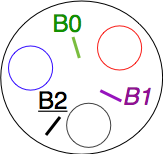
\includegraphics[width=0.2\textwidth]{philosophes}
  \caption{\label{fig:philosophes}Problème des philosophes}
\end{wrapfigure}
Le problème des philosophe est résumé sur la figure \ref{fig:philosophes}.
Chacun veut saisir la baguette de droite et de gauche qui sont chacune partagée avec (respectivement) son voisin de gauche et de droite.

Le problème est que si tout le monde commence par prendre la baguette de gauche, il n'y a plus de baguette de droite disponible (puisqu'elle est à gauche de votre voisin de droite) et donc on se trouve dans une impasse.
Il s'agit d'un \textbf{\textit{deadlock}}.
Un programme est en situation de \textbf{\textit{deadlock}} lorsque tous ses threads d'exécution sont bloqués et qu'aucun d'entre eux ne peut être débloqué sans exécuter d'instructions d'un des threads bloqués.
La seule façon de sortir d'un programme dans une situation de deadlock, est de l'arrêter complètement et de le redémarrer.
C'est donc un problème grave !\\
Attention : Les tests successifs ne permettent pas toujours de détecter les deadlock, il se peut qui ne se produise qu'après un temps assez long.


\paragraph{Une solution au problème des philosophes} serait d'ordonnée les baguettes (leurs assigner un numéro par exemple), et de faire en sorte que les philosophes les prennent toujours dans le même ordre comme présenté ci-dessous.
Cette solution fonctionne néanmoins il faut être conscient qu'avec cette solution il est possible qu'un seul philosophe ne mange alors que tout les autres attendent, ce qui est une perte de performance énorme lorsqu'il y a beaucoup de philosophe!
\begin{lstlisting}
void* philosophe ( void* arg )
{
  int *id=(int *) arg;
  int left = *id;
  int right = (left + 1) % PHILOSOPHES;
  while(true) {
    // philosophe pense
    if(left<right) {
      pthread_mutex_lock(&baguette[left]);
      pthread_mutex_lock(&baguette[right]);
    }
    else {
      pthread_mutex_lock(&baguette[right]);
      pthread_mutex_lock(&baguette[left]);
    }
    mange(*id);
    pthread_mutex_unlock(&baguette[left]);
    pthread_mutex_unlock(&baguette[right]);
  }
  return (NULL);
}
\end{lstlisting}


Ce problème des philosophe est à l'origine de la règle de bonne pratique suivante : Pour éviter les deadlocks, il est nécessaire d'ordonnancer tous les mutex utilisés par le programme dans un ordre struct.
Lorsqu'un thread doit réserver plusieurs  mutex en même temps, il doit \textit{toujours} effectuer ses appels à \texttt{pthread\_mutex\_lock} dans l'ordre choisi pour les mutex.
(Sinon deadlock possible).

\subsubsection{Les sémaphores}
Il s'agit d'une autre solution au problème de la coordination entre threads.
Un \textbf{\textit{sémaphore}} est une structure de données qui est maintenue par l'OS et contient :
\begin{itemize}
  \item Un entier qui stocke la valeur, $\geq 0$, du sémaphore
  \item Une queue qui contient les pointeurs vers les threads qui sont bloqués en attente sur le sémaphore.
\end{itemize}

L'implémentation d'un sémaphore contient 4 fonctions principale :
\begin{itemize}
  \item Une fonction d'initialisation du sémaphore (\texttt{int sem\_init(sem\_t *sem, int pshared, unsigned int value);}).
  \item Une fonction permettant de détruire le sémaphore et libérer les ressources associées (\texttt{int sem\_destroy(sem\_t *sem);}).
  \item Une fonction \texttt{post} qui permet d'incrémenter la valeur du sémaphore ou de débloquer un thread en attente (s'il y en a un).
    (\texttt{int sem\_post(sem\_t *sem);}).
  \item Une fonction \texttt{wait} qui permet de tester la valeur du sémaphore, si elle est $>0$, décrémente le sémaphore et continue, sinon bloque le thread et attend qu'un autre thread fasse un \texttt{post}.
    (\texttt{int sem\_wait(sem\_t *sem);}).
\end{itemize}

Dans le cadre de ce cours ne nous limitons au sémaphore POSIX.
Pour pouvoir les utiliser il faut importer \texttt{semaphore.h} qui contient les différentes signatures (dont celle reprisent dans la liste ci-dessus) et la structure de données de type \texttt{sem\_t}.


\paragraph{Exclusion mutuelle}~\\
Les sémaphores permettent de résoudre le problème de l'exclusion mutuelle.
En fait lorsque le sémaphore est initialisé à \texttt{1}, on peut l'utiliser de manière semblable à un mutex.
Néanmoins il y a des différences importantes : Un sémaphore est conçu pour être manipulé par différents threads et il est très possible qu'un thread exécute \texttt{sem\_wait} et qu'un autre exécute \texttt{sem\_post}.
Pour les mutex, certaines implémentations supposent que c'est le même thread qui exécute le \texttt{lock} et le \texttt{unlock}.
Lorsque ces opérations doivent être effectuées dans des threads différents,e il est donc préférable d'utiliser des sémaphores à la place des mutex.

\paragraph{Problème du rendez-vous}~\\
Ce problème est rencontré lorsqu'une application découpé en $N$ thread doit attendre la fin de l'exécution d'une première phase dans les $N$ threads avant de pouvoir passer à la suite.
Chaque thread peut être résumé par une 1e phase, suivit d'un endroit de "rendez-vous" pour tous les threads et d'une deuxième phase.
La solution est la suivante :
\begin{lstlisting}
premiere_phase();

pthread_mutex_lock(&mutex);		//section critique pour count
count++;
if(count==N) {					// si tous les threads sont arrives
  sem_post(&rendezvous);
}
pthread_mutex_unlock(&mutex);	//fin de section critique
sem_wait(&rendezvous);			//attente a la "barriere"
sem_post(&rendezvous);			//liberation d'un autre thread en attente

seconde_phase();
\end{lstlisting}
Cette solution permet de résoudre le problème du rendez-vous avec un nombre fixe de threads\footnote{Certains implémentations de la librairie threads POSIX implémentent une barrière similaire à la solution ci-dessus.
  Une barrière est une structure de données de type \texttt{pthread\_barrier\_t}.
  Elle s'initialise en utilisant la fonction \texttt{pthread\_barrier\_init} qui prend 3 arguments : un pointeur vers une barrière, des attributs optionnels et le nombre de threads qui doivent avoir atteint la barrière pour que celle-ci s'ouvre.
  La fonction \texttt{pthread\_barrier\_destroy} permet de détruire une barrière.
Enfin, la fonction \texttt{pthread\_barrier\_wait} qui prend comme argument un pointeur vers une barrière.}.

\paragraph{Problème des producteurs-consommateurs}~\\
Soit une application découpé en deux types de threads (dont le nombre n'est pas connu ni fixe à priori) :
\begin{itemize}
  \item les \textit{producteurs} : Produisent des données et placent le résultat dans une zone mémoire accessible aux consommateurs.
  \item les \textit{consommateurs} : Utilisent les données produitent par les producteurs.
\end{itemize}
Ces deux types de threads communiquent en utilisant un buffer qui a une capacité limité à $N$ slots comme sur la figure \ref{fig:prodcons}
\begin{figure}[h!]
  \centering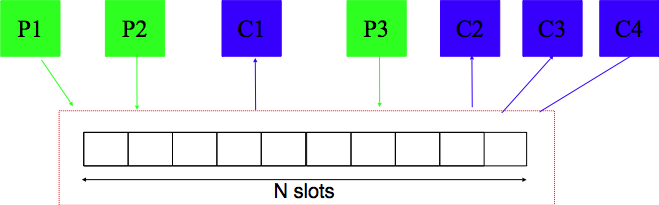
\includegraphics[width=0.5\textwidth]{prodcons}
  \caption{\label{fig:prodcons}Problème des producteurs-consommateurs}
\end{figure}
Le buffer étant partagé, il est nécessaire d'utiliser un mutex pour protégé son accès.
Un producteur ne doit être bloqué que si tout le buffer est rempli et inversement un consommateur ne doit être bloqué que si tout le buffer est vide.
Le problème peut être résolu avec 2 sémaphores comme le montre les extraits de codes ci-dessous.
\begin{lstlisting}
...
// Dans la fonction principale : Initialisation
#define N 10 // nbre de slots du buffer
pthread_mutex_t mutex; 	sem_t empty; sem_t full;

pthread_mutex_init(&mutex, NULL);
sem_init(&empty, 0 , N);  // empty compte le nbre de slot vide => N = buffer vide
sem_init(&full, 0 , 0);   // full compte le nbre de slot rempli => 0 = buffer vide
...
// Le Producteur
void producer(void){
  int item;
  while(true){
    item=produce(item);
    sem_wait(&empty); 				// attente d'un slot libre
    pthread_mutex_lock(&mutex);  	// section critique
    insert_item();
    pthread_mutex_unlock(&mutex);	// fin de section critique
    sem_post(&full); 				// il y a un slot rempli en plus
  }
}

// Le Consommateur
void consumer(void){
  int item;
  while(true){
    sem_wait(&full); 				// attente d'un slot rempli
    pthread_mutex_lock(&mutex); 		// section critique
    item=remove(item);
    pthread_mutex_unlock(&mutex);
    sem_post(&empty); // il y a un slot libre en plus
  }
}
\end{lstlisting}

\paragraph{Problème des readers-writers}~\\
Soit de nouveau une application découpé en deux types de threads (dont le nombre n'est pas connu ni fixe à priori) :
\begin{itemize}
  \item les lecteurs (\textit{readers}) qui lisent des données partagées mais ne les modifie pas.
  \item les écrivains (\textit{writers}) qui modifient des données partagées.
\end{itemize}
Plusieurs \textit{readers} peuvent lire en même temps, mais lorsqu'un writers modifie les données, il ne peut ni avoir d'autre \textit{writers} ni de \textit{readers} qui utilisent les données.
Lorsqu'on cherche une solution à ce problème il faut faire attention à ne pas donner priorité aux \textit{readers} (ce qui serait plus simple).
Une solution au problème est présentée dans les extraits de codes ci-dessous\footnote{Certaines implémentations de la librairie threads POSIX contiennent des Read-Write locks qui s'appuie sur des sémaphore pour résoudre le problème des readers-writers…}.
\begin{lstlisting}
/* Initialisation */
pthread_mutex_t mutex_readcount; 	// protege readcount
pthread_mutex_t mutex_writecount; 	// protege writecount
pthread_mutex_t z; 					// un seul reader en attente
sem_t wsem;       					// acces exclusif a la db
sem_t rsem;							// pour bloquer des readers
int readcount=0;
int writecount=0;
sem_init(&wsem, 0, 1);
sem_init(&rsem, 0, 1);

/* Writer */
while(true){
  think_up_data();
  pthread_mutex_lock(&mutex_writecount);	// section critique - writecount
  writecount=writecount+1;
  if(writecount==1) {						// si c'est le premier writer qui arrive
    sem_wait(&rsem);
  }
  pthread_mutex_unlock(&mutex_writecount);// fin de la section critique - writecount
  sem_wait(&wsem);						// section critique, un seul writer a la fois
  write_database();
  sem_post(&wsem);						// fin de la section critique
  pthread_mutex_lock(&mutex_writecount);	// section critique - writecount
  writecount=writecount-1;
  if(writecount==0) {						// depart du dernier writer
    sem_post(&rsem);
  }
  pthread_mutex_unlock(&mutex_writecount);// fin de la section critique - writecount
}

/* Reader */
while(true){
  pthread_mutex_lock(&z);					// 1e exclusion mutuelle, un seul reader en attente sur rsem
  sem_wait(&rsem);

  pthread_mutex_lock(&mutex_readcount);	// exclusion mutuelle, readercount
  readcount=readcount+1;
  if (readcount==1) {						// si arrivee du premier reader
    sem_wait(&wsem);
  }
  pthread_mutex_unlock(&mutex_readcount);	// fin exclusion mutuelle, readercount
  sem_post(&rsem);  						// liberation du prochain reader
  pthread_mutex_unlock(&z);				// fin 1e exclusion mutuelle
  read_database();
  pthread_mutex_lock(&mutex_readcount);	// exclusion mutuelle, readcount
  readcount=readcount-1;
  if(readcount==0) {						// si depart du dernier reader
    sem_post(&wsem);
  }
  pthread_mutex_unlock(&mutex_readcount);	// fin exclusion mutuelle, readcount
  use_data_read();
}
\end{lstlisting}


\section{Processus}
Un \textbf{\textit{processus}} peut être défini comme étant une instance de programme qui est en train d'être exécuté sur un ou plusieurs processeurs sous le contrôle d'un système d'exploitation.
Un processus comprend donc un ensemble d'instructions pour le processeur, les données qui sont stockées en mémoire et un ou plusieurs (si plusieurs threads) contextes.
En outre, l'OS maintient un certain nombre de structure de données qui sont nécessaires au bon fonctionnement du processus.
Ces structures de données sont créées au démarrage du processus, mises à jour durant la vie du processus puis supprimées lorsque le processus s'arrête.

\subsection{Les librairies}
Lorsqu'un programme s'exécute à l'intérieur d'un processus, il exécute des instructions de différentes "origines" :
\begin{itemize}
  \item Les instructions écrites par le programmeur, provenant d'un ou de plusieurs module et regroupée dans un exécutable.
  \item Les instructions des librairies standard du système.
\end{itemize}
Si on analyse la compilation avec gcc, on constatera que le code des librairies standard ne sont pas inclus mais que seul les appels aux fonctions y sont indiqués.
Cela explique la taille réduite des exécutables sous Linux et de nombreuses variantes Unix.
Un programme peut utiliser deux types de librairies :
\begin{itemize}
  \item une \textbf{librairie statique} (\textit{static library}) est une librairie de fonctions qui est intégrée directement avec le programme.
    Elle fait entièrement partie de l'exécutable. \\
    Avantage : Portabilité. Désavantage : Poids
  \item une \textbf{librairie partagée} (\textit{shared library}) est un ensemble de fonctions qui peuvent être appelées par un programme mais sont stockées dans un seul fichier sur le disque.
    Ce fichier unique est utilisé automatiquement par tous les programmes qui utilisent des fonctions de la librairie.\\
    Avantage : Poids, pas de copies inutiles.
\end{itemize}

Il est parfois intéressant de créer une librairie qui peut être liée de façon statique, par exemple pour une exécution sur un autre ordinateur. Pour ce faire il faut compiler les fichiers objet correspondant aux différents modules de la librairie (avec \texttt{gcc}). Ensuite il faut regrouper les différents modules dans une archive qui constituera la librairie. Par convention , toutes les librairies ont un nom qui commence par \texttt{lib} et se termine par l'extension \texttt{.a}. Sous Linux,cette opération est réalisée par l'utilitaire \texttt{ar}\footnote{Voir page de manuel. En bref : \texttt{ar r libname.a module.o} permet l'ajout d'un module objet. \texttt{ar d libname.a module.o} permet la suppression d'un module objet d'une librairie et \texttt{ar tv libname.a} permet de lister le contenu de la librairie}.

L'archive contenant la librairie peut être liée en utilisant le linker à n'importe quel programme qui en utilise une ou plusieurs fonctions. Avec \texttt{gcc} ça donne par exemple ça : \texttt{gcc --static -g -o executable libname.a exemple.o}. L'argument \texttt{--static} force le compilateur à inclure le code de la librairie dans l'exécutable. \\

Lorsqu'un programme est compilé de façon à utiliser une librairie dynamique, c'est l'OS qui analyse le programme lors de son chargement et intègre automatiquement les fonctions des librairies qui sont nécessaires à son exécution. L'entête de l'exécutable contient de l'information générée par le compilateur qui permet de localiser les librairies dynamiques qui doivent être intégrées\footnote{L'utilitaire \texttt{ldd} permet de lister les librairies partagées d'un exécutable}.
\subsection{Les appels système}
\begin{figure}[h!]
  %\begin{wrapfigure}{r}{0.4\textwidth}
  %\vspace{-0.5cm}
  \centering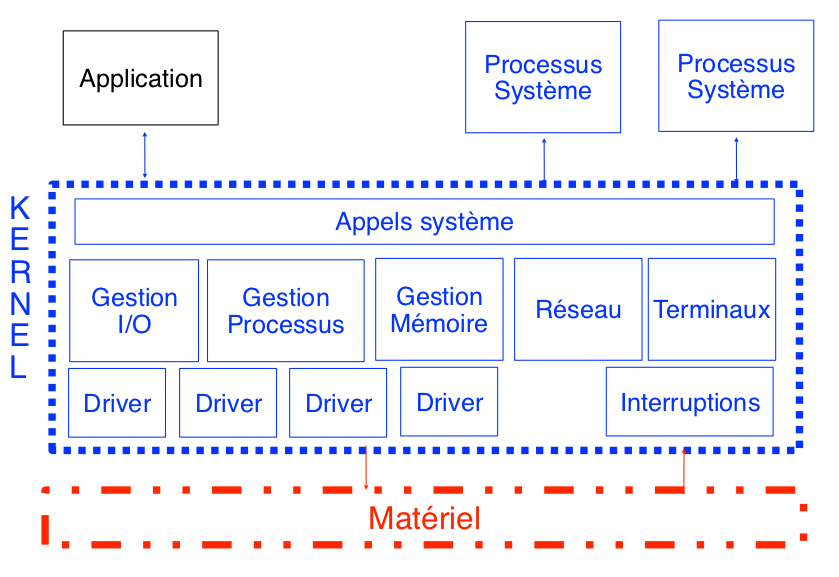
\includegraphics[width=0.6\textwidth]{appelssystemes}
  \caption{\label{fig:appelssystemes}Appels systèmes}
  %\vspace{-0.5cm}
  %\end{wrapfigure}
\end{figure}

Outre l'utilisation de fonctions de librairies, les programmes doivent interagir avec l'OS.
Un OS tel qu'Unix contient des utilitaires tels que \texttt{ls}, \texttt{grep},...
et un noyau ou \textit{kernel}.
Le \textit{\textbf{kernel}} contient les fonctions de base du système d'exploitation qui lui permet à la fois d'interagir avec le matériel et de gérer les processus en mémoire.
Parmi les fonctions de bases, il y en a un petit nombre (de quelques dizaines à quelques centaines) qui sont utilisable par les processus lancés par les utilisateurs.
Ce sont les appels système.
Un \textbf{\textit{appel système}} est une fonction du \textit{kernel} qui peut être appelée par n'importe quel processus.
Pour un appel système on a :
\begin{enumerate}
  \item Appeler le kernel.\\
    L'adresse de retour est automatiquement sauvegardée sur la pile lors de l'instruction qui fait appel au kernel (comme avec \texttt{calll}).
  \item Quel appel système ? \\
    Le numéro de l'appel système est placé dans le registre \texttt{\%eax}, cela permet à la routine de l'OS de savoir de quel appel système il s'agit
  \item Passer les arguments \\
    Sous Linux, les arguments d'un appel système sont placés par convention dans des registres.
    Sur IA32, le 1e argument est placé dans le registre \texttt{\%ebx}, le 2e dans \texttt{\%ecx},...
    Ce qui permet au kernel de facilement récupérer les arguments d'un appel système en lisant le contenu des registres.
  \item Exécuter appel système
  \item Retourner le résultat\\
    À la fin de l'appel système, le résultat est placé dans \texttt{\%eax}.
    Et \texttt{errno} est mis à jour en cas d'échec.
  \item Retour au processus appelant
\end{enumerate}

Les processeurs actuels fonctionnent au minimum avec deux modes :
\begin{itemize}
  \item le \textbf{mode utilisateur} où quelques instructions spécifiques de manipulation du matériel et certaines adresses mémoires ne sont pas utilisable.
  \item le \textbf{mode protégé} ou toutes les instructions du processeur et toutes les adresses mémoires sont utilisables
\end{itemize}
Le noyau de l'OS s'exécute en mode protégé tandis que les processus utilisateurs s'exécutent en mode utilisateur.
Ces derniers ne peuvent donc pas directement exécuter les instructions permettant une interaction avec des dispositifs matériel; pour cela il faut passer par l'OS.

Lorsqu'un utilisateur démarre, le processeur est placé en mode protégé et le kernel se charge. Il initialise différentes structures de données et lance \texttt{init} qui est le 1e processus du système. Dès que \texttt{init} a été lancé, le processeur passe en mode utilisateur et exécute les instructions de ce processus. Après cette phase de démarrage, les instructions du kernel seront exécutées lorsque une interruption matérielle surviendra ou qu'un processus utilisateur exécutera un appel système. L'interruption matérielle place automatiquement le processeur en mode protégé et le kernel exécute la routine de traitement d'interruption correspondant à l'interruption qui est apparue. Un appel système démarre par l'exécution d'une instruction spéciale (parfois appelée \textit{interruption logicielle}) qui place le processeur en mode protégé et puis démarre l'exécution d'une instruction placée à une adresse spéciale en mémoire\footnote{Sur certains processeurs de la famille IA32, c'est l'instruction \texttt{int 0x80}, sur d'autre c'est \texttt{syscall} qui permet ce passage du mode utilisateur vers le mode protégé}.

\subsection{Création d'un processus}
Considérons par exemple un utilisateur qui exécute la commande \texttt{/usr/bin/expr 1 + 2} depuis un shell \texttt{bash} interactif. Pour exécuter cette commande, il faut exécuter un nouveau processus contenant les instructions assembleur se trouvant dans \texttt{/usr/bin/expr}, lui passer les arguments \texttt{1 + 2}, l'exécuter, récupéré sa valeur de retour et la retourner au shell qui pourra l'utiliser et poursuivre son exécution. Les designers de Unix ont choisis de construire un appel système pour chacune de ces opérations\footnote{Cet appel système est défini dans \texttt{unistd.h}} : \texttt{pid\_t fork(void)}. Après exécution de \texttt{fork}, il y a 2 copies du même processus en mémoire. Le processus qui a appelé \texttt{fork} est le \textit{processus père}, tandis que celui qui a été crée est le \textit{processus fils}. L'appel de \texttt{fork} retournera deux valeurs différentes aux processus père et au processus fils :
\begin{itemize}
  \item \texttt{0} pour le processus fils
  \item \texttt{>0} pour le processus père. Cette valeur correspond à l'identifiant du processus fils crée.
  \item \texttt{-1} en cas d'erreur. Dans ce cas, \texttt{errno} est mis à jour.
\end{itemize}
Contrairement au thread, les données en mémoires sont toutes copiée et donc même la modification d'une variable globale ou d'une zone mémoire n'aura aucun impact sur l'autre processus. (Pour connaître les moyens de communication entre processus, voir la section \ref{communicationproc} à la page \ref{communicationproc}). \\

Le kernel gère les processus et attribue un identifiant (de type \texttt{pid\_t} sous Unix) à chaque processus. L'appel système \texttt{gitpid} permet de récupérer l'identifiant du processus courant tandis que \texttt{getppid} permet de récupérer l'identifiant du processus père. \\

Après l'appel de \texttt{fork}, les 2 processus partagent certaines ressources qui sont gérée par le kernel. Notamment \textit{stdin}, \textit{stdout} et \textit{stderr}. Il faut donc que des précaution soit prise afin que les écritures sur la sorties standard s'affiche correctement (par exemple). En réalité les fonctions telles que \texttt{printf} et \texttt{putchar} de la librairie standard utilisent l'appel système \texttt{write} qui est le seul permettant d'écrire sur un flux tel que \textit{stdout}. L'utilisation à outrance de cet appel système est coûteux pour les performance d'une application, c'est pourquoi, la librairie standard utilise un buffer dans laquelle elle stocke temporairement les données avant de les écrire en une fois via \texttt{write}\footnote{Ce buffer peut être contrôlé avec \texttt{setvbuff} et \texttt{setbuf}. Par exemple pour le désactiver : \texttt{setbuf(stdout, NULL}}. Il est possible de "vider"\footnote{C'est à dire de forcer l'écriture sur le flux concerné.} immédiatement le buffer en utilisant la fonction \texttt{\textbf{int} fflush(\textbf{FILE} *stream)}.

\subsection{Fin d'un processus}
Comme nous l'avons déjà vu, un programme C peut se terminer de 2 façons :
\begin{itemize}
  \item par l'exécution de \texttt{return ...}  dans la fonction \texttt{main}.
  \item par un appel explicite à \texttt{exit(...)}
\end{itemize}
Ces fonctions utilisent en fait la fonction de la librairie \texttt{exit}. Il est possible de définir une ou plusieurs fonctions à exécuter lors de la terminaison d'un processus en utilisant \texttt{\textbf{int} atexit(\textbf{void} (*function)(\textbf{void}));}. De cette manière, lorsque \texttt{exit} est appelé, elle lance d'abord les fonctions de terminaisons définies puis termine correctement le processus. Cela est utile, par exemple, lorsqu'un processus utilise une mémoire partagée entre plusieurs processus afin de libérer les ressources. Ensuite l'appel système \texttt{exit} est appelé : C'est le seul appel système qui n'a pas de valeur de retour. Cet appel système permet au processus qui se termine de retourner un statut à son processus père. Pour récupéré ce statut, un processus père doit utiliser l'appel système \texttt{waitpid} via  \texttt{\textbf{pid\_t} waitpid(\textbf{pid\_t} pid, \textbf{int} *status, \textbf{int} options);}. Cet appel système est un appel système bloquant. Si le pid passé en 1e argument est négatif, cela signifiera qu'on attend n'importe quel processus fils. \\
Un processus qui lance un processus fils avec \texttt{fork} \textit{doit} attendre la terminaison de son processus fils en utilisant \texttt{waitpid}. Différents macros tels que \texttt{WEXISTATUS} et \texttt{WTERMSIGN} peuvent être utilisées (\texttt{WEXISTATUS} pour extraire la valeur de retour et \texttt{WTERMSIGN} pour extraire la raison de la terminaison abrupte), ils sont décrits en détail dans \texttt{man waitpid}. \\

Lorsque le père se termine avant le processus fils, le processus fils est dit \textbf{\textit{orphelin}} et le kernel lui attribue l'identifiant \texttt{1} (correspondant à \texttt{init}) comme père. Un \textit{\textbf{processus zombie}}, quant à lui, est un processus qui s'est terminé mais dont la valeur de retour n'a pas encore été récupérée par son père\footnote{Dans ce cas le kernel libère l'ensemble des ressources du processus fils et ne conserve qu'une petite structure de donnée contenant entre autre : son identifiant, l'identifiant du père, et sa valeur de retour. En pratique, il faut éviter \^{}\^{}}.

\subsection{Exécution d'un programme}
Pour exécuter un programme, il existe l'appel système \texttt{execve}. Celui-ci remplace l'image en mémoire du processus par l'image de l'exécutable passé en argument, et son exécution démarre à la fonction \texttt{main} de ce dernier.\\
\texttt{\textbf{int} execve(\textbf{const} \textbf{char} *path, \textbf{char} *\textbf{const} argv[], \textbf{char} *\textbf{const} envp[]);}\\
\texttt{execve} ne retourne un valeur de retour que en cas d'échec, en effet dans le cas contraire, tout ce qui se trouve après \texttt{execve} ne sera pas exécuté puisque tout est remplacé par le nouveau programme. Dans le cas d'un processus ayant lancé des threads, ceux-ci seraient automatiquement supprimé puisque c'est toute l'image qui est remplacée. Par contre pour les flux standard (\textit{stdout},..), il est préférable de forcer leur écriture avec \texttt{fflush} car ce n'est pas fait automatiquement.\\

Les valeurs retourné par un processus fils sont stockée sur 8 bits, la plus grande valeur positive est donc 127 (utilisé en cas d'erreur ?). \\

En C, il existe des variantes à \texttt{execve} : \texttt{execl}, \texttt{execp}, \texttt{execle} et \texttt{execv}. Celle-ci diffèrent de \texttt{execve} par leur manière de spécifier les arguments. \\
La fonction \texttt{sytem} de la librairie permet d'exécuter une commande du shell directement depuis un programme.\\

En plus des exécutable compilé, Unix et Linux supporte aussi l'exécution de \textit{programmes interprétés}. %Un \textbf{\textit{programme interprété}} est un programme écrit dans un langage qui doit être utilisé via un \textit{interpréteur}.
Un \textit{\textbf{interpréteur}} est un programme qui lit des commandes sous la forme de texte et exécute directement les instructions correspondant à ces commandes. Le plus connu est \texttt{bash} mais citons également \texttt{awk} (manipulation de textes), \texttt{perl} (textes mais aussi d'autres applications), \texttt{python} (langage de programmation complet). \\

Voyons comment \texttt{execve} fonctionne :
\begin{enumerate}
  \item Vérifie que le programme est bien exécutable : Le système de fichier contient des métadonnés, dont un bit\footnote{En pratique 3 bits, en fonction de l'utilisateur : voir \ref{sysfichierutilisateur} page \pageref{sysfichierutilisateur}} de permission qui indique si le fichier est exécutable ou non.
  \item Vérifie le type de fichier : Par convention le début d'un fichier contient une séquence d'octets ou de caractère qui indiquent le type de fichier dont il s'agit\footnote{Ce type de fichier peut être testé avec la commande \texttt{file}}.
    \begin{enumerate}[a)]
      \item Soit il s'agit d'un fichier directement exécutable.
        Sous les systèmes Linux actuels, ce fichier sera au format \texttt{elf}
        et début par une entête qui contient une chaîne de caractère
        utilisée comme marqueur ou chaîne magique.
      \item Soit le fichier est en langage interprété et débute alors par \texttt{\#!} suivit du nom complet de l'interpréteur à utiliser et de ses paramètres éventuels à utiliser.
    \end{enumerate}
\end{enumerate}
En pratique, on peut définir n'importe quel interpréteur (et en créer), il suffit qu'il s'agisse d'un exécutable. Celui-ci recevra le texte du fichier à interpréter. Cette facilité d'ajouter de nouveaux interpréteur de commande est une des forces des OS de la famille Unix.

\subsection{Table des processus}
Un OS tel que Linux maintient certaines infos à propos de chaque processus dans une \textbf{\textit{table de processus}}. Ces infos peuvent être obtenue via \texttt{ps}, \texttt{top},\texttt{pstree},... En fait tout ces utilitaire utilisent les informations contenue dans le répertoire \texttt{/proc}. Ce répertoire contient plusieurs entrée (fichiers et répertoires). Citons le répertoire \texttt{/proc/\textit{pid}/} où \texttt{\textit{pid}} est l'identifiant du processus. Ce répertoire contient notamment :
\begin{itemize}
  \item \texttt{cmdline} : Ligne de commande de lancement
  \item \texttt{environ} : Variables d'environnements
  \item \texttt{status} : État actuel du processus , Identifiant, identifiant du père,...
  \item \texttt{limits} : Limites actuelles imposées par le système pour le processus.
  \item \texttt{task} : Répertoire qui contient pour chaque thread lancé par le processus un sous-répertoire avec les infos sur le thread.
  \item \texttt{maps} : représente de famon textuelle la table des segments de mémoire qui sont partagés
\end{itemize}

\section{Communications entre processus}
\label{communicationproc}
Pour la communication entre processus on peut utiliser un \textit{pipe} s'il ont un ancêtre commun, ou une \textit{fifo}. Une \textit{fifo} peut être créée en utilisant la commande \texttt{mkfifo} ou la fonction \texttt{mkfifo} qui s'utilise comme l'appel système \texttt{open}. Pour créer une nouvelle \textit{fifo} il suffit de lui donner un nom (chaîne de caractère), tout processus connaissant ce nom pourra l'utiliser.
\subsection{Signaux}
Un \textit{signal} est une forme d'interruption logicielle. Un \textit{\textbf{signal}} Unix est un mécanisme qui perment à un processus de réagir de façon asynchrone à un événement qui s'est produit. Il en existe 2 types :
\begin{itemize}
  \item \textit{signal synchrone} : directement causé par l'exécution d'une instruction du processus. Par exemple, le signal \texttt{SIGFPE} qui est généré par l'OS quand un processus provoque une exception lors du calcul d'expression mathématique (ex : div par 0).
  \item \textit{signal asynchrone} : Cause externe au processus. (ex : provoqué par \texttt{kill})
\end{itemize}
L'OS prévoit par défaut le traitement de tous les signaux, mais il est possible de redéfinir ce traitement avec l'appel système \texttt{signal} qui permet d'associé un \textit{handler} à chaque signal. Unix permet également d'envoyer un signal avec l'appel système \texttt{kill}.\\
\begin{tabularx}{\textwidth}{l|p{0.615\textwidth}|c}
  \textbf{Signal} & \textbf{Provoqué lorsqu'une} & \textbf{Par défaut} \\
  \hline \hline
  \texttt{SIGALRM} & Une alarme définie par la fonction \texttt{alarm} ou \texttt{setitimer} a expiré. & Terminaison \\
  \hline
  \texttt{SIGBUS} & Erreur au niveau matériel & Terminaison \\
  \hline
  \texttt{SIGSEGV} & Erreur dans l'accès à la mémoire & Terminaison \\
  \hline
  \texttt{SIGFPE} & Erreur au niveau de l'utilisation des fonction mathématiques &  Terminaison \\
  \hline
  \texttt{SIGTERM} & Utilisé par défaut par \texttt{kill} pour demandé la fin du processus & Terminaison \\
  \hline
  \texttt{SIGKILL} & Pour forcer la terminaison. Ne peut être redéfini et ignoré. & Terminaison \\
  \hline
  \texttt{SIGUSR1} et \texttt{SIGUSR2} & Peuvent être utilisés par des processus sans conditions particulière & Terminaison \\
  \hline
  \texttt{SIGCHLD} & Indique qu'un processus fils s'est arrêté ou a fini son exécution. & Ignoré \\
  \hline
  \texttt{SIGHUP} & À l'origine, pour indiquer que la connexion avec le terminal avait été rompue. Parfois utiliser par des processus serveur pour indiquer qu'il faut recharger leur fichier de config & ? \\
  \hline
  \texttt{SIGINT} & envoyé lorsqu'on tape \texttt{Ctrl-C} dans un shell & Terminaison \\
  \hline
\end{tabularx}

\subsubsection{Envoi de signaux}
\texttt{\textbf{int} kill(\textbf{pid\_t} pid, \textbf{int} sig);}\\
\texttt{pid} peut être :
\begin{itemize}
  \item > 0 : Le \texttt{pid} du processus.
  \item = 0 : Pour tout les processus du même groupe de processus\footnote{Par défaut un processus appartient au même groupe que son parent. L'appel système \texttt{setpgid} permet de le changer. En pratique c'est fait par le shell lorsqu'on utilise les pipes \texttt{|} afin de pouvoir arrêter tout les processus avec Ctrl-C si nécessaire.}.
  \item = -1 : Pour tout les processus pour lesquels le processus à les permissions d'envoyer un signal
  \item < -1 : Pour tout les processus qui font partie du groupe \texttt{-pid}
\end{itemize}
\subsubsection{Traitement de signaux}
2 appels systèmes sont possibles pour spécifier comment un signal doit être traité : \texttt{signal} et \texttt{sigaction}. \\
\texttt{\textbf{typedef} \textbf{void} (*\textbf{sighandler\_t})(\textbf{int});\\
\textbf{sighandler\_t} signal(\textbf{int} signum, \textbf{sighandler\_t} handler);}\\
Pour spécifié le traitement par défaut on utilise \texttt{SIG\_DFL} en argument, en pour ignorer le signal \texttt{SIG\_IGN}. \texttt{signal} renvoit l'ancienne \textit{handler} utilisée ou \texttt{SIG\_ERR} en cas d'erreur.\\

Il faut être attentif à ce que la fonction handler puisse bien s'exécuter à n'importe quel moment de l'exécution (alors que d'autres instructions était en cours d'exécution). Il n'est cependant pas possible d'utiliser les mutex pour les signaux car il faut que le traitement du signal soit terminé pour qu'on puisse retourné à la fonction dans laquelle on se trouvait. Il est important de déclarer les variables globale utilisé par la gestion du signal comme étant \texttt{volatile} afin de forcer à recharger la valeur avant chaque utilisation. Mais cela ne suffit pas car un signal peut interrompre le processus juste après qu'il ait rechargé la valeur et juste avant qu'il ne l'utilise. C'est pourquoi il est préférable de n'utiliser que des variables du type \texttt{sig\_atomic\_t} qui garantit que les accès se feront de manière atomique. Il faut également être attentif à ne pas utiliser des fonctions de la librairies standard qui pourrait interférer avec elles même si elles sont en cours d'utilisation par le processus principal (par exemple si le handler modifie \texttt{errno}, alors qu'on l'utilise déjà). \\

Pour le traitement des signaux par un OS, il y a 2 stratégies :
\begin{itemize}
  \item Considérer qu'un signal est un message envoyé par la noyau ou un processus à un autre processus. Le noyau contient une queue qui stocke tous les signaux destinés à un processus donné. Chaque fois que le noyau réactive une processus, il vérifie si la queue associé contient un ou plusieurs messages concernant des signaux, si c'est le cas il appel la fonction de traitement du signal.\\
    Avantage : Tout les signaux sont reçu.\\
    Inconvénient : Il faut maintenir une queue de taille variable pour chaque processus.\\
  \item Représenter l'ensemble des signaux qu'un processus peut recevoir sous la forme de drapeaux binaires (1 drapeau par signal). Avec cette stratégie, lors de l'envoi d'un signal, on modifie le drapeau correspondant sur le processus destination (sauf si ce processus ignore ce type de signal). Chaque fois que le noyau réactive un processus, il vérifie les drapeaux relatifs aux signaux du processus. Si un drapeau est vrai il appel la fonction de traitement correspondante. \\
    Avantage : Il suffit d'un bit par signal. \\
    Inconvénient : Aucune garantie sur la délivrance des signaux. Le nombre de signaux reçu n'est pas fiable.
\end{itemize}
La plupart des variantes de Unix utilisent la 2e stratégie. \\

Un \textbf{\textit{appel système lent}} est un appel système dont l'exécution peut être interrompue par la réception d'un signal. (Exemples : \texttt{sleep}, \texttt{read},..). Lorsqu'un signal survient pendant l'exécution d'un tel appel système, celui-ci est automatiquement interrompu pour laisser place au traitement du signal et est terminé ensuite en retournant une erreur et en mettant \texttt{errno = EINTR}.

\subsubsection{Traitement de signaux asynchrones}
Après réception d'un signal asynchrones, il faudrait pouvoir continuer le code autre part que là où il s'est arrêté. Pour ce faire on a les fonctions \texttt{int setjmp(jmp\_buf env);} et \texttt{int sigsetjmp(sigjmp\_buf env, int savesigs);}. Voici un exemple de leur utilisation :
\begin{lstlisting}
#include ...
sigjmp_buf buf;
static void sigfpe_handler(int);

int main (int argc, char *argv[]){
  if(signal(SIGFPE,sigfpe_handler)==SIG_ERR) {
    perror("signal");
    exit(EXIT_FAILURE);
  }
  for(int i=1;i<argc;i++) {
    char *endptr; int r;
    long val=strtol(argv[i],&endptr,10);
    if(*endptr=='\0') {
      r=sigsetjmp(buf,1);						// faut-il ignorer le resultat ?
      if(r==0){
        int resultat=1252/(int) val;
        printf("1252/%d=%d\n",(int) val,resultat);
      }
      else {
        printf("%d/%d=NaN\n",n,(int) val);
      }
    }
    else{
      printf("Argument incorrect : %s\n",argv[i]);
    }
  }
  return(EXIT_SUCCESS);
}

static void sigfpe_handler(int signum){
  siglongjmp(buf,1);								// ignorer la donnee
}
\end{lstlisting}
\subsubsection{Temporisateurs}
Il est possible d'envoyer un signal après un certain temps en utilisant \texttt{setitimer} ou \texttt{alarm} afin d'arrêter un appels systèmes bloquant après un certain temps. Exemple (si on veut laisser que 5 seconde à l'utilisateur pour taper 1 caractère de réponse):
\begin{lstlisting}
...
if(signal(SIGALRM, sig_handler)==SIG_ERR)==SIG_ERR){ perror("signal"); exit(EXIT_FAILURE); }
if(siginterrupt(SIGALRM,true)<0){	// Indique qu'il faut arreter les appels systemes si on recoit SIGALRM
  perror("siginterrupt"); exit(EXIT_FAILURE);
}
...
char c;
alarm(5);
int r = read(STDIN_FILENO, &c, 1);
if((r==1)){
  alarm(0); 			// reset timer
  ...					// On utilise la reponse donnee
} else {
  ... 				// On utilise une valeur par defaut
}
...

static void sig_handler(int signum){
  // rien a faire, read sera interrompu
}
\end{lstlisting}
Si le système est surchargé, il est possible qu'il y ait 5 secondes qui passe entre la ligne 8 et la ligne 9. Pour éviter ce problème il faudra donc faire appel à \texttt{siglongjmp} et \texttt{sigsetjmp} afin de savoir si un signal \texttt{SIGALRM} a déjà été reçu.
\subsection{Sémaphores}
Il n'est pas possible d'utiliser la fonction \texttt{sem\_init} vue de le cas des threads car les processus ne partagent pas nécessairement la même zone mémoire. Par contre, il est possible d'utilisé un sémaphore nommé. Un \textbf{\textit{sémaphore nommé}} est identifié par un \textit{nom}; sous Linux, il correspond à un fichier (dans le dossier virtuel \texttt{/dev/shm} et tout processus qui connaît le nom et a les autorisation d'y accéder peut l'utiliser. \\
\texttt{\textbf{sem\_t} *sem\_open(\textbf{const char} *name, \textbf{int} oflag);\\
  \textbf{sem\_t} *\textbf{sem\_open}(\textbf{const char} *name, \textbf{int} oflag, \textbf{mode\_t} mode, \textbf{unsigned int} value);\\
  \textbf{int} sem\_close(\textbf{sem\_t} *sem);\\
\textbf{int} sem\_unlink(\textbf{const char} *name);}\\
En cas d'erreur, \texttt{sem\_open} retourne \texttt{SEM\_FAILED} et met à jour \texttt{errno}. Les sémaphores nommés peuvent être créés et supprimés comme des fichiers. Ils utilisent des ressources limités, il faut donc bien le supprimer (avec \texttt{sem\_unlink} une fois qu'il n'est plus nécessaire.

\subsection{Partage de fichiers}
Comme l'écriture dans un fichier sur un dispositif de stockage est relativement lent, l'OS maintient un buffer qui permet de ne pas devoir attendre l'écriture réelle sur le dispositif avant de continuer le processus. Pour forcer l'écriture de ce buffer sur le dispositif, on peut utiliser l'appel système \texttt{fsync} (ou \texttt{sync} si on veut le faire pour toutes les données).\\

Lors de l'ouverture d'un fichier sous Unix, le kernel maintient une structure de données (\textit{open file object}) qui contient le mode, l'offset pointeur, la référence vers le fichier sur le système d'exploitation. Lorsque 2 programme ouvre un même fichier, il possède chacun un \textit{open file object} différent tandis que si un fichier est ouvert avant un \texttt{fork}, le père et le fils possède le même \textit{open file object}. Ce qui peut poser problème si on déplace l'offset pointeur. Pour éviter ce problème il faut utiliser \texttt{\textbf{ssize\_t} pread(\textbf{int} fd, \textbf{void} *buf, \textbf{size\_t} count, \textbf{off\_t} offset);} et \texttt{\textbf{ssize\_t} pwrite(\textbf{int} fd, \textbf{const void} *buf, \textbf{size\_t} count, \textbf{off\_t} offset);} qui garantissent que les opérations d'écriture et de lecture qui sont effectupes se font de manière atomique et donc à l'offset pointeur voulu.\\

Il existe aussi un système de \textit{lock} similaires aux mutex. En théorie il existe 2 techniques :
\begin{itemize}
  \item \textit{mandatory locking} : C'est l'OS qui vérifie qu'aucun accès fait au fichier ne viole les locks.
  \item \textit{advisory locking} : C'est le processus qui doit vérifier
\end{itemize}
Certains Unix supporte le mandatory locking mais la plupart ne supportent que l'advisory locking (qui est la plus facile à implémenter et est la plus performante). \\
Il existe deux appels systèmes : \texttt{\textbf{int} flock(\textbf{int} fd, \textbf{int} operation);} (et \texttt{fcntl}). \texttt{operation} peut prendre les valeurs :
\begin{itemize}
  \item \texttt{LOCK\_SH} : Lock partagé : Plusieurs processus peuvent posséder un même lock vers le fichier.
  \item \texttt{LOCK\_EX} : Lock exclusif.
  \item \texttt{LOCK\_UN} : Pour supprimer un lock.
\end{itemize}
L'appel système \texttt{fcntl} et la fonction \texttt{flock} sont plus flexible et permette de placer des locks sur une partie de fichier.\\

Le noyau maintient pour chaque fichier ouvert une liste de locks. Sous linux, on peut visualiser l'état de ces locks avec \texttt{cat /proc/locks}. À noter que \texttt{EOF} indique la fin du fichier.



\section{Fichiers et répertoires}

\subsection{Gestion des utilisateurs}
Unix est un OS multi-utilisateur ce qui impose des contraintes de sécurités :
\begin{itemize}
  \item il doit être possible d'identifier et/ou d'authentifier les utilisateurs
  \item il doit être possible d'exécuter des processus appartenant à plusieurs utilisateurs simultanément et de déterminer quel utilisateur est responsable de chaque opération.
  \item l'OS doit fournir des mécanismes simple de contrôle d'accès aux différentes ressources (mémoire, stockage,...)
  \item il doit être possible d'allouer certaines ressources à un utilisateur particulier à un moment donné
\end{itemize}

Les systèmes Unix utilise le processus \texttt{login} pour la connexion d'un utilisateur. Ce processus appartient initialement à \textit{root} puis exécute l'appel système \texttt{setuid} afin d'appartenir à l'utilisateur puis exécute \texttt{execve} pour lancer le premier shell de l'utilisateur. L'appel système \texttt{setuid} ne peut évidemment être appelé que par un processus appartenant à \texttt{root}. Un processus peut récupéré son \textit{userid} avec l'appel système \texttt{getuid}.\\

Sur Unix, le fichier \texttt{/etc/passwd} contient pour chaque utilisateur : le nom d'utilisateur (username), le mot de passe (sur les anciennes versions de Unix), l'identifiant de l'utilisateur (\textit{userid}), l'identifiant de son groupe principal, son nom et son prénom, son répertoire de démarrage, son shell.\\

En pratique, on associe parfois des droits d'accès à un groupe d'utilisateur plutôt qu'à un utilisateur particulier. Le groupe principal d'un utilisateur est définit dans \texttt{/etc/passwd} tandis que les groupe secondaires le sont dans \texttt{/etc/group}.
\subsection{Systèmes de fichiers}
Tout les dispositifs de stockage (disque dur, lecteur CD/DVD, clé USB,...) offrent en pratique une interface similaire pour le système d'exploitation. Cette interface se résume en 2 fonction, une de lecture d'un secteur et un de l'écriture. En règle général, un \textit{\textbf{secteur}} peut stocker un bloc de 512 octets. Chaque secteur est identifié par une adresse. La plupart des implémentations sont optimisées pour pouvoir lire ou écrire plusieurs secteurs consécutifs, mais la plus petite unité de lecture ou d'écriture est le \textit{secteur}. La plupart des OS (dont Unix) fournissent une interface de plus haut niveau aux programme : les fichiers et répertoire. Cette abstraction est appelée un \textit{\textbf{système de fichiers}} ou \textit{filesystem}. Il existe des centaines de système de fichiers; Linux en supporte quelques dizaines. \\

En simplifiant, un système de fichier Unix utilise le principe qu'un \textit{fichier} est une suite ordonnée d'octets. Un nom est associé à cette suite d'octets. Cette suite d'octets sera stockée dans un ou plusieurs secteurs, consécutif ou non. Rien ne garantit que la taille d'un fichier sera un multiple du nombre d'octets dans un secteur, donc l'OS doit être capable de gérer des secteurs partiellement rempli.\\

Sous Unix, le lien entre les différents secteurs qui composent un fichier se fait grâce à l'utilisation d'inodes. Un \textit{\textbf{inode}} est une structure de données stockée sur le disque (en pratique un ensemble contigu de secteur, souvent au début du disque) et qui contient notamment les méta-informations d'un fichier suivantes :
\begin{itemize}
  \item \texttt{uint16 mode} : Contient un ensemble de drapeaux binaires avec les permissions associées au fichier
  \item \texttt{uid\_t uid} : Le propriétaire du fichier
  \item \texttt{gid\_t gid} : Le groupe auquel appartient le fichier
  \item \texttt{uint32 size} : La taille du fichier en bytes.
  \item \texttt{uint32 atime} : L'instant de dernier accès
  \item \texttt{uint32 mtime} : L'instant de dernier modification
  \item \texttt{uint32 ctime} : L'instant de création
  \item \texttt{uint16 nlinks} : Le nombre de liens vers ce fichier
  \item \texttt{uint16 zone[10]} . La liste ordonnée des secteurs qui contiennent le fichier.
\end{itemize}
Sous Unix, le nom de fichier n'est pas directement associé au fichier lui-même, il est stocké dans les répertoires. Un \textit{repertoire} est un fichier qui a un format spécial. Il contient une suite d'entrées qui contiennent chacune un nom (de fichier ou de répertoire), une indication de type (qui permet notamment de distinguer fichiers et répertoires) et le numéro de l'inode qui contient les méta-données du fichier ou répertoire concerné. \\

Dans un système de fichier Unix, l'ensemble des répertoires et fichiers est organisé sous la forme d'un arbre. La racine de cet arbre est le répertoire \texttt{/}. Le système de fichier Unix permait aussi d'intégrer facilement des systèmes de fichiers se trouvant sur différents dispositifs de stockage. Cela peut se faire en pratique par un administrateur système avec la commande \texttt{mount} ou via le fichier \texttt{/etc/fstab}. \\

Tout répertoire contient 2 répertoires spéciaux : \texttt{.} qui est un alias vers le répertoire lui-même, et \texttt{..} qui est un alias vers le répertoire parent du répertoire courant. \\

\subsubsection{Permissions}
\label{sysfichierutilisateur}
Les métadonnées qui sont associés à chaque fichier ou répertoire contiennent des bits de permissions pour 3 types de permissions et d'autorisation : \texttt{r} = lecture, \texttt{w} = écriture/modification et \texttt{x} = exécution.
Ces bits de permissions sont regroupés en 3 blocs : les permissions applicable par un processus de l'utilisateur propriétaire, les permissions applicables par un processus appartenant au même groupe que le fichier et les permissions applicables par les autres processus. Ces bits de permissions peuvent être modifié par la commande \texttt{chmod}\footnote{Voir note page 177 du syllabus pour plus d'information sur les représentation des bits de permission et l'utilisation de \texttt{chmod}}. \\

\subsubsection{Répertoire courant}
Un processus peut utiliser le nom complet d'un fichier commençant par \texttt{/} (\texttt{/home/damien/Bureau/exemple.txt}) ou son nom \textit{relatif} (\texttt{Bureau/exemple.txt}). Pour les noms relatif, en fait le kernel maintient pour chaque processus le \textit{répertoire courant} dans sa table des processus. Par défaut, il s'agit du répertoire à partir duquel le programme a été lancé. Un processus peut changer son répertoire avec l'appel système \texttt{\textbf{int} chdir(\textbf{const} \textbf{char} *path);}\footnote{Depuis le shell on utilise la commande \texttt{cd} pour changer de répertoire, et la commande \texttt{pwd} pour connaître le répertoire courant}.

\subsubsection{Appels systèmes}
\begin{itemize}
  \item \texttt{stat} : permet de récupérer les métadonnées d'un fichier ou un répertoire.\\
    $\Rightarrow$ Commande \texttt{stat}
  \item \texttt{chmod} et \texttt{chown} : Permet de modifier respectivement le mode (permissions) et le propriétaire ou le groupe d'un fichier.\\
    $\Rightarrow$ Commande \texttt{chmod}, \texttt{chown} et \texttt{chgrp}
  \item \texttt{utime} : Permet de modifier un timestamp associés à un fichier/répertoire. \\
    $\Rightarrow$ Commande \texttt{touch}
  \item \texttt{rename} : Permet de changer le nom d'un fichier / répertoire\\
    $\Rightarrow$ Commande \texttt{rename}
  \item \texttt{mkdir} et \texttt{rmdir} : Permet de créer / supprimer un répertoire\\
    $\Rightarrow$ Commande \texttt{mkdir} et \texttt{rmdir}
  \item \texttt{opendir}, \texttt{closedir} et \texttt{readdir} : Permettent de consulter le contenu d'un répertoire.
  \item \texttt{link} et \texttt{unlink} : Permet de créer ou supprimer des "liens" vers un fichier. Le compteur de lien \texttt{nlinks} est mis à jour pour l'inode en question. Lorsqu'un inode ne contient plus de lien, il est supprimé. \\
    $\Rightarrow$ Commande \texttt{ln} et \texttt{rm}
\end{itemize}

\subsubsection{Utilisation des fichiers}
Lorsqu'un processus veut accéder à un fichier il peut utiliser les appels systèmes \texttt{open}, \texttt{read} / \texttt{write} et \texttt{close}. (Il est également possible d'utiliser les fonctions \texttt{fopen}, \texttt{fread}, \texttt{fwrite} et \texttt{fclose} proposé par la librairie standard). \\
\texttt{\textbf{int} open(\textbf{const char} *pathname, \textbf{int} flags); \\
\textbf{int} open(\textbf{const char}* pathname, \textbf{int} flags, \textbf{mode\_t} mode);} \\
\texttt{flags} peut prendre une valeur parmi
\begin{itemize}
  \item \texttt{O\_RDONLY}, \texttt{O\_WRONLY} et \texttt{O\_RDWR}
  \item \texttt{O\_CREAT}, \texttt{O\_APPEND}, \texttt{O\_TRUNC}, \texttt{O\_CLOSEXEC}\footnote{Spécifique à Linux, si le fichier doit être automatiquement fermé lors de l'exécution de \texttt{execve}.}, et \texttt{O\_SYNC}\footnote{Indique que les opérations d'écriture doivent être faites immédiatement sans être mises en attente dans les buffers du kernel}.
  \item Une disjonction logique (opérateur \texttt{|}) des entre les drapeaux précédents
\end{itemize}
Lors de l'exécution de \texttt{open} (et uniquement à ce moment là), l'OS vérifie si le processus a les permissions suffisante pour accéder au fichier. Si c'est le cas, l'OS l'ouvre et retourne un \textit{descripteur de fichier}. Sous Unix, un \textbf{\textit{descripteur de fichier}} est représenté sous la forme d'un entier positif : \texttt{open} retournera le plus petit descripteur de fichier disponible. Par convention, \texttt{0} = \textit{stdin}, \texttt{1} = \textit{stdout}, \texttt{2} = \texttt{stderr}. Toutes les opérations qui sont faites sur un fichier se font en utilisant le \textit{descripteur de fichier} comme référence au fichier. Un \textit{descripteur de fichier} est une ressource limité dans un OS tel qu'Unix, il faut donc les fermer en fin d'utilisation et ne pas ouvrir inutilement un grand nombre de fichier. Pour fermer : \\
\texttt{\textbf{int} close(\textbf{int} fd);}\\
Par défaut l'OS ferme les descripteur \texttt{0}, \texttt{1} et \texttt{2} à la fermeture d'un processus. \\

Lorsqu'un fichier a été ouvert, le kernel maintient les références vers l'\textit{inode} du fichier ainsi qu'un \textit{offset pointer} qui indique la position actuelle de la tête de lecture/écriture. Il est possible de déplacer cet offset pointeur en utilisant l'appel système \texttt{lseek} : \\
\texttt{\textbf{off\_t} lseek(\textbf{int} fd, \textbf{off\_t} offset, \textbf{int} whence);}\\
L'argument \texttt{whence} permet de définir si la position doit être calculé de manière absolue (\texttt{SEEK\_SET}) ou s'il faut l'additionner avec la valeur actuelle (\texttt{SEEK\_CUR}), ou s'il faut l'additionner à la fin du fichier (\texttt{SEEK\_END}).\\

Pour lire et écrire on dispose de 2 fonctions : \\
\texttt{\textbf{ssize\_t} read(\textbf{int} fd, \textbf{void} *buf, \textbf{size\_t} count);}\\
\texttt{\textbf{ssize\_t} write(\textbf{int} fd, \textbf{const} \textbf{void} *buf, \textbf{size\_t} count);}\\
Ces 2 fonctions permettent d'écrire des séquence contigües d'octets. Lorsqu'un fichier est envoyé via internet (par exemple), et lu sur un autre ordinateur cela peut poser plusieurs problèmes :
\begin{itemize}
  \item Les ordinateurs n'utilisent pas spécialement tous le même nombre d'octets pour représenté un certain type de donnée\footnote{Sur un ancier IA32, les entiers sont représentés sur 32 bits = 4 bytes, sur les plus récent, ils sont représentés sur 64 bits = 8 bytes}.
  \item Les fabricants de processeurs utilisent plusieurs techniques pour représenter les entiers sur 16 et 32 bits en mémoire (figure \ref{fig:biglittleendian})
    \begin{itemize}
      \item le \textit{big endian} (utilisé sur les PowerPC).
      \item le \textit{little endian} (utilisé sur les processeurs IA32).
    \end{itemize}
\end{itemize}
\begin{figure}[!h]
  \centering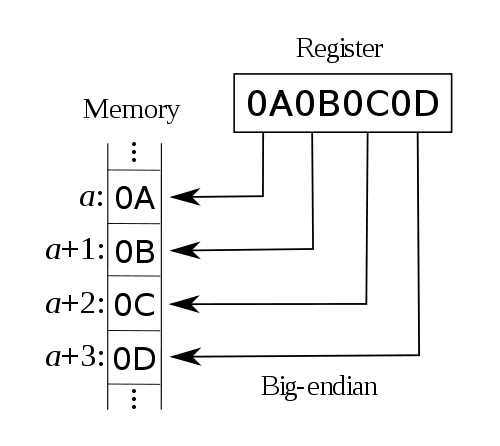
\includegraphics[width=0.3\textwidth]{bigendian}
  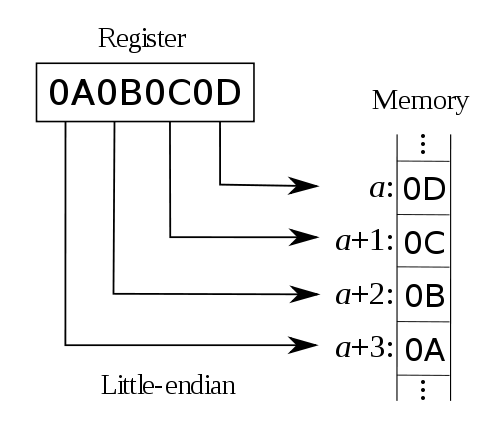
\includegraphics[width=0.3\textwidth]{littleendian}
  \caption{\label{fig:biglittleendian} Big-endian et little-endian}
\end{figure}

Note : Il est possible d'obtenir un nom de fichier unique à partir d'un template en utilisant la fonction \texttt{ \textbf{int} mkostemp (\textbf{char} *template [, \textbf{int} flags]);}. En utilisant \texttt{unlink} directement après la création du fichier, cela supprime le fichier du système de fichier mais il reste accessible par le processus qui l'a ouvert $\Rightarrow$ fichier temporaire.


\subsubsection{Les pipes}
Un \textit{\textbf{pipe}} est un flux de bytes unidirectionnel qui relie deux processus qui ont un ancêtre commun. L'un des processus écrit sur le \textit{pipe}, tandis que l'autre peut lire sur le \textit{pipe}. Un \textit{pipe} est crée en utilisant l'appel système \texttt{pipe} : \\
\texttt{\textbf{int} pipe(\textbf{int} fd[2])}\\
Chaque fois qu'une donnée est écrite sur \texttt{fd[1]}, elle peut être lue avec \texttt{fd[0]}.
Un \textit{pipe} a une capacité limitée\footnote{4 kB sur Linux <2.6.11 x86-32, 64 kB sur Linux > 2.6.11} lorsqu'un pipe est rempli, le processus qui effectue \texttt{write} est bloqué.


En pratique les pipes sont utilisés par le shell avec \texttt{|}. Exemple : \texttt{cat exemple.txt | grep "word"}. La sortie standard de \texttt{cat} est relié avec l'entrée standard de \texttt{grep}.

\section{Mémoire virtuelle}
\subsection{La mémoire virtuelle}
\begin{wrapfigure}{r}{0.4\textwidth}
  \vspace{-0.5cm}
  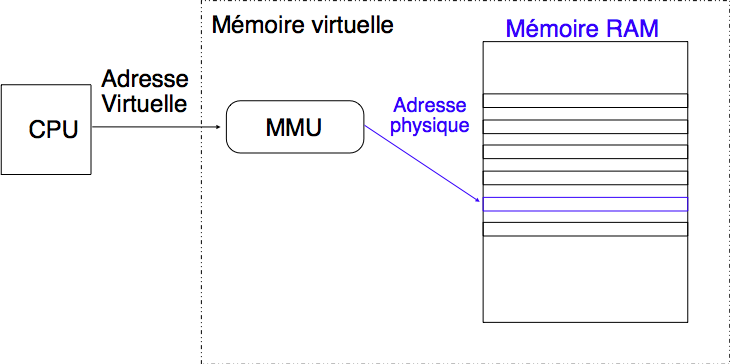
\includegraphics[width=0.5\textwidth]{mmu}
  \caption{\label{fig:mmu}\textit{MMU} et mémoire virtuelle}
\end{wrapfigure}
Avec la \textit{\textbf{mémoire virtuelle}}, deux types d'adresse sont utilisées su le système : Les \textit{adresses virtuelles} et les adresse réelles ou physiques. Une \textit{\textbf{adresse virtuelle}} est une adresse qui est utilisée à l'intérieur d'un programme.  Une \textit{\textbf{adresse physique}} est l'adresse qui est utilisée au niveau des puces de RAM pour les opérations d'écriture et de lecture. Ce sont les adresses physiques qui sont échangées sur le bus auquel la mémoire est connectée. \\
Le rôle du \textit{\textbf{MMU}} ou \textbf{\textit{Memory Management Unit}} est de traduire les adresse virtuelles en adresse physiques. \\

La longueur des adresses virtuelles et des adresses physiques ne doit pas nécessairement être de la même. Sur les ordinateurs bons marchés par exemple, les adresses virtuelles sont plus longues; ils utilisent une quantité réduite de mémoire RAM. Inversement on peut utiliser des adresses physiques plus langues que les adresses virtuelles (sur les serveurs par exemple).\\

Un autre avantage de la mémoire virtuelle est qu'elle permet, à condition de pouvoir avoir une conversion spécifique à  chaque processus, de partager efficacement la mémoire entre processus tout en leur permettant d'utiliser les mêmes adresses virtuelles. \\
Le \textit{MMU} est capable d'effectuer des traductions d'adresses virtuelles spécifiques à chaque processus ce qui permet non seulement que 2 adresses virtuelles identiques pointe vers 2 adresses physiques différentes mais aussi que 2 adresses virtuelles différentes puisse pointer vers 1 adresse physique (utile pour éviter de copier les librairies partagées) \\
\subsection{La mémoire virtuelle}
\begin{wrapfigure}{r}{0.5\textwidth}
  \vspace{-0.5cm}
  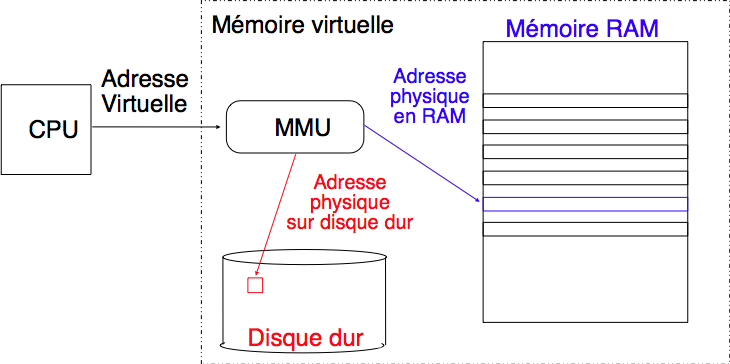
\includegraphics[width=0.5\textwidth]{memvirt}
  \caption{\label{fig:memvirt}Organisation de la mémoire virtuelle}
\end{wrapfigure}
Un autre avantage encore est la possibilité de combiner mémoire RAM et dispositif de stockage (disque dur, disque SSD,...) pour obtenir une mémoire virtuelle de plus grande capacité que la mémoire RAM.

\subsubsection{Fonctionnement de la mémoire virtuelle}
La difficulté de gestion est que la mémoire est organisé en octet tandis que les dispositifs de stockage utilisent des secteurs de données. Le temps d'accès diffèrent également.\\

(ici je comprends pas trop dans le syllabus... j'ai l'impression qu'il manque une partie)\\

Lorsqu'un programme est chargé en mémoire (\texttt{execve}), il est automatiquement découpé en pages. Ces pages peuvent être stockée dans n'importe quelle zone de la mémoire RAM mais doivent être à des adresses qui sont contiguës. Une \textit{adresse virtuelle} est alors composée d'un ensemble de bits. Les bits de poids fort identifient la \textit{page}, tandis que ceux de poids faible identifient la position de la donnée par rapport au début de cette \textit{page}.\\
\begin{figure}
  \centering
  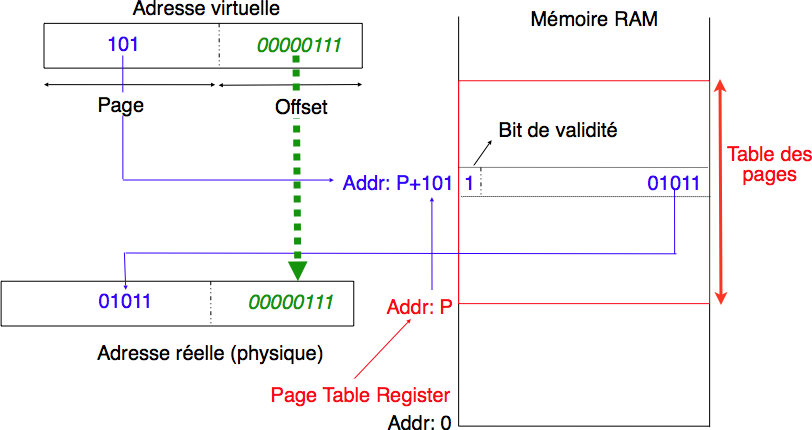
\includegraphics[width=0.5\textwidth]{memtradadresses}[!h]
  \caption{Traduction d'adresses avec une table des pages}
\end{figure}\\
Avec ce principe de \textit{pages}, un mécanisme de traduction d'adresses peut se baser sur une \textit{\textbf{table de pages}}. Cette \textit{table de pages} est stockée en mémoire RAM et contient une ligne pour chaque page existant dans la mémoire virtuelle. Cette table de page contient :
\begin{itemize}
  \item le \textit{\textbf{bit de validité}} qui indique si la page est en mémoire RAM ou non
  \item l'adresse en mémoire RAM à laquelle la page est actuellement stockée (si elle est en RAM).
  \item des bits de permission géré par l'OS : \textit{R} bit (lecture), \textit{W} bit (écriture) et \textit{X} bit (exécution)
\end{itemize}

L'adresse de la table des pages est stockés dans un registre du processeur.
L'utilisation de ce registre permet d'avoir une table des pages pour chaque processus.
Pour cela il suffit qu'une zone de mémoire soit réservée pour chaque processus
et que l'OS y stocke la table des pages du processus.
Lors du changement de contexte, l'OS modifie alors le registre de la table des pages.

En terme de sécurité,
il faut éviter qu'un processus ne puisse modifier sa table des pages
lui-même sans contrôle. Pour ce faire on utilise les bits de permissions.
Un segment de code qui ne contient que des instructions sera par exemple
stocké avec les bits \textit{R} et \textit{X} mais pas le bit \textit{W}.
Le stack par contre sera placé dans des pages avec les bits \textit{R}
et \textit{W} mais pas \textit{X}.
Un accès interdit à une pages provoquera une segmentation fault.

Les bits de permissions sont gérées par l'OS mais il peut parfois être utile de la modifier pour certaines pages. Cela se fait avec \texttt{\textbf{int} mprotect(\textbf{const void} *addr, \textbf{size\_t} len, \textbf{int} prot)} où \texttt{prot} peut prendre les valeurs \texttt{PROT\_NONE}, \texttt{PROT\_READ}, \texttt{PROT\_WRITE}, \texttt{PROT\_EXEC} ou une disjonction logique de ceux-ci. Si la protection demandé est plus \textit{faible} que celle actuelle, l'OS produira une segmentation fault.

La traduction se fait comme suit

\begin{enumerate}
  \item L'adresse virtuelle arrive au MMU, il regarde combien de bits de
    points faibles on a
    (si une page fait \si{4}{KiB}, ça fait $2^{12}$ bytes
    donc 14 bits de points faibles.)
    Les bits de point fort donnent l'indice dans la table des pages en binaire
    (11001 signifie que c'est la 25ème entrée de la table des page).
  \item Le MMU regarde si la partie de la table des pages où il y a l'entrée
    25 est dans la TLB (sorte de cache pour la table des pages).
    Dans tous les cas, il regarde dans la table des pages,
    l'entrée à l'indice 25.
  \item Il regarde le bit de validité de l'entrée.
    \begin{itemize}
      \item Si c'est 1, c'est que c'est dans la RAM,
        il regarde alors les bits de permission pour voir s'il a le droit
        de faire ce qu'il veut faire (lire, écrire ou exécuter)
        (sinon, segfault).
        Il met le bit de réference à 1 et il regarde les autres bits pour voir
        à quel multiple de la taille d'une page, la page est.
        Par exemple, si ça vaut 1011, c'est que c'est à l'adresse physique
        $11\cdot 2^{12}$ (avec des pages de \si{4}{KiB}).
        S'il a écrit dedans, il met le dirty bit à true.
      \item Si c'est 0,
        il regarde les bits de permission, s'ils sont tous à false,
        c'est que la page est invalide (segfault),
        sinon, c'est que la page est sur le disque,
        il regarde s'il a les permissions, s'il ne les a pas segfault.
        Sinon, il ramène la page dans la RAM et met le dirty bit à false
        (pour dire que pour l'instant, la page est exactement pareil dans
        la RAM que dans la swap donc si il faudra par la suite la remettre
        dans la swap, il faudra même pas faire de copie)
        puis il met le bit de référence à true et s'il écrit,
        il met le dirty bit à true aussi.
    \end{itemize}
  \item Une fois qu'il a l'adresse physique de début de la page,
    il ajoute à ça l'offset (les bits de point faibre de l'adresse virtuelle)
    et il a l'adresse physique exacte :)
\end{enumerate}

Tous les $x$ temps, il remet les bits de références à faux.

Il ne faut pas confondre ça avec \lstinline{mmap}

\begin{itemize}
  \item Quand la RAM déborde,
    l'OS met les pages les moins utilisées sur le disque dans une partition
    swap ou un fichier de swap
    (celle qui ont le bit de référence à faux et dirty bit à faux
    en préférence car ça veut dire qu'elles ont pas été utilisées
    récemment et qu'elle sont déjà en swap de manière inchangée).
    Quand on a à nouveau besoin de cette page, on la remet en RAM.
  \item \lstinline{mmap} prend de la mémoire dans le
    système de fichier (file system)
    et la met dans le heap en RAM.
    Mais si le système a besoin de place,
    il peut très bien la remettre sur le disque.
    À ce moment là,
    je sais pas trop s'il la remettra où elle était avant
    (c'est à dire dans le système de fichier)
    (il le fera sans doute s'il est malin) ou s'il la met en swap.
\end{itemize}

\subsubsection{Mémoire partagée}
Il est possible qu'une même page en mémoire physique soit utilisé par plusieurs processus différents. Par exemple dans le cas des threads (crées par l'OS), lorsqu'on crée un thread, on initialise sa table de page en copiant toutes les valeurs de son "père" mis à part celle qui correspond au stack. De cette manière le thread a accès au même variable global, segment text,... \\

En utilisant la table des pages intelligemment il est également possible de permettre à deux processus distincts d'avoir accès à la même zone mémoire physique. Ce qui leurs permettra de communiquer plus efficacement qu'avec des pipes par exemple. Cette technique porte le nom de \textit{\textbf{mémoire partagée}}. Pour ce faire 2 technique existent :
\begin{itemize}
  \item L'OS copie la table des pages du processus $P1$ dans la table des pages de $P2$.
  \item L'OS créer une nouvelle page pouvant être partagée. Elle appartient au noyau mais est accessible à $P1$ et $P2$ en modifiant leur table des pages. \\
    Avantages : meilleur contrôle possible par l'OS + peut vivre après la terminaison d'un processus.
\end{itemize}
Linux utilise la 2e solution. La mémoire partagée peut y être utilisée avec les appels système \texttt{shmget} (pour créer ou vérifier l'accès), \texttt{shmat} (pour ajouter la mémoire à la table des pages) et \texttt{shmdt} (pour détacher un segment de mémoire).\\

\begin{wrapfigure}{r}{0.3\textwidth}
  \vspace{-0.5cm}
  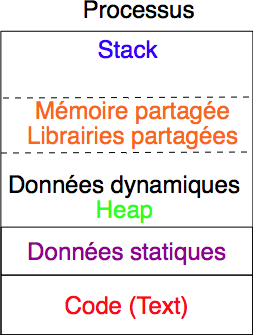
\includegraphics[width=0.3\textwidth]{mempart}
  \caption{\label{fig:mempart}Organisation de la mémoire d'un processus}
\end{wrapfigure}
Il faut faire attention au pointeur en mémoire partagé ! En pratique, il ne vaut mieux pas les utiliser...\\

Les segments de mémoire partagée sont gérés par le noyau, ils persistent donc après la terminaison du processus qui les a crée. Le nombre de segments partagés est limité. Il ne faut donc pas qu'il y en ai qui restent alors qu'ils ne sont plus utilisé. Il est possible de supprimer un segment partagé en utilisant l'appel système \texttt{shmctl}. En pratique, le noyau détruit un segment de mémoire partagée uniquement lorsqu'il n'y a plus de processus qui y sont attachés. On peut donc faire cette suppression juste après \texttt{shmat} de manière à être sûr que le segment sera supprimé si plus aucun processus n'est actif dessus (utilisable par exemple si on utilise la mémoire partagée pour communiquer entre un processus père et un fils).


\subsubsection{Implémentation de fork}
Afin d'optimiser le fonctionnement de fork, il n'y a pas de réelle copie des pages du processus père. En réalité le système utilise \textit{copy-on-write}. Le noyau copie toutes les entrées de la table des pages du processus père vert la table des pages du processus fils et les marque d'un bit $p$ pour indiquer qu'elles sont en \texttt{copy-on-write}.  Si un processus tente un accès en écriture sur une de ces pages, le MMU interrompt l'exécution du processus et force l'exécution d'une routine d'interruption du noyau. Si le processus a effectivement les autorisation d'écriture, le noyau alloue une nouvelle page physique et y recopie la page  où la tentative a eu lieu. La table des pages est mises à jour et le processus peut continuer. Cette technique de \textit{\textbf{copy-on-write}} permet de ne copier que les pages qui sont effectivement modifiées par le processus père ou le processus fils.
\subsection{Fichiers mappés en mémoire}
\begin{figure}[!h]
  \centering 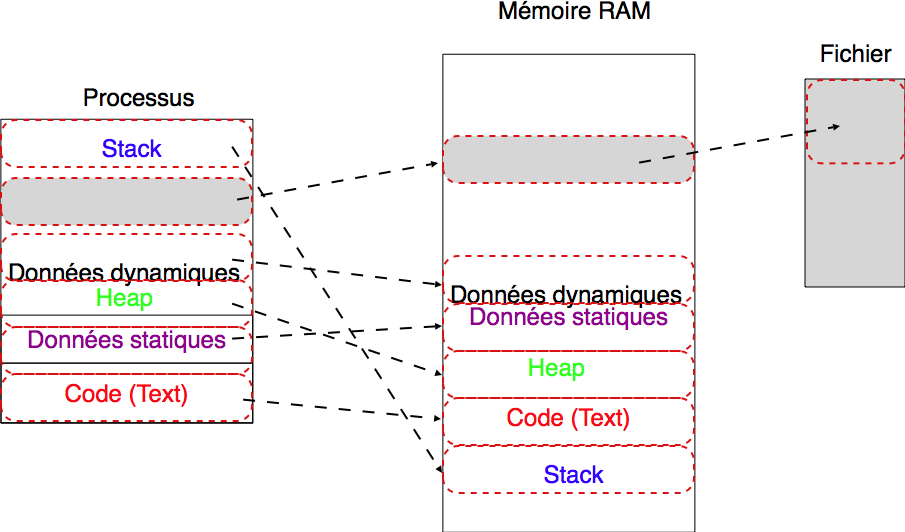
\includegraphics[width=0.7\textwidth]{mmap}
  \caption{\label{fig:mmap}Fichier mappés en mémoire}
\end{figure}
Grâce à la mémoire virtuelle il est possible de placer le contenu d'un fichier ou une partie dans une zone de mémoire du processus. Cette opération peut être effectuée en utilisant l'appel système \texttt{mmap}. \texttt{mmap} prend entre autre un argument qui spécifie si les pages du fichier sont mappées dans chaque processus (avec \texttt{MAP\_PRIVATE} dans ce cas une écriture n'est pas répercuté sur les autres processus) ou si plusieurs processus peuvent accéder et modifier la page (avec \texttt{MAP\_SHARED}). Les changements fait sur un fichier mappés ne sont pas immédiatement fait dans le fichier sur le dispositif de stockage. On peut utiliser \texttt{msync} permet de demander cette écriture doit être faite (avec le drapeau \texttt{MS\_SINC} il attend la fin, tandis qu'avec \texttt{MS\_ASYNc} il ne fait que démarrer l'écriture). \\
À la fin de l'utilisation, d'un fichier mappé, le processus doit appeler l'appel système \texttt{munmap}.
\subsection{Utilisation des dispositifs de stockage}
Comme nous l'avions vu plus haut, les pages peuvent ne pas se trouver en mémoire RAM. Dans ce cas, soit elles n'existe plus, soit elles sont stockée sur un dispositif de stockage. Sous Linux on utilise une partition \textit{swap} pour stocké les pages qui ne sont pas en mémoire RAM. Le fonctionnement de la mémoire virtuel peut alors être vu de la façon suivante : le \textit{MMU} est intérgré directement sur le processeur et comprend un \textit{TLB} (\textit{Translation Lookaside Buffer}) qui sert de cache pour les entrées de la table des pages du processus qui est en train de s'exécuter. Si la page demandé ne se trouve pas en mémoire RAM, il s'occupera de la rapatrié (ce qui peut prendre quelque dizaine de millisecondes). Tant que cette page n'est pas disponible en mémoire RAM, le processus est mis à l'état bloqué et l'OS effectue un changement de contexte pour exécuter un autre processus.
\subsection{Stratégie de remplacement de pages}
C'est l'OS qui prend en charge le transferts des pages entre les dispositifs de stockage et la mémoire. Tant que la RAM n'est pas remplie, il suffit de ramener une ou plusieurs pages du dispositif de stockage vers la mémoire RAM.  En général, l'OS utilisera le principe de localité. Par contre si la mémoire RAM est pleine, il faut une stratégie de remplacement des pages.

Une première stratégie de remplacement de pages pourrait être de sauvegarder les identifiants des pages dans une file \textit{FIFO}. C'est facile à implémenter mais les premières pages arrivées ne sont pas spécialement les moins utilisée.

Une autre stratégie serait de maintenir les statistiques d'utilisation de chaque page afin de prédire les pages qui seront nécessaires dans le futur. Mais cette stratégie nécessiterait que le \textit{TLB} mette à jour les statistique à chaque accès à une page : difficile, et pas performant.

Face à ces problèmes, la plupart des stratégies de remplacement de pages s'appuient sur 2 bits qui se trouvent dans chaque entrée de la table des pages. C'est facilement implémentable et ça n'augmente pas trop la mémoire occupée par une entrée de la table des pages.
\begin{itemize}
  \item le \textit{bit de référence} est mis à vrai par le \textit{MMU} dans le \textit{TLB} à chaque accès (r/w) à une donnée se trouvant dans la page en question.
  \item le \textit{bit de modification} ou \textit{dirty bit} est mis à vrai par le \textit{MMU} chaque fois qu'une opération d'écriture est réalisée.
\end{itemize}
Lorsqu'une entrée de la table des pages est retirée du \textit{TLB}, que ce soit à l'occasion d'un changement de contexte ou parce que le \textit{TLB} était plein, les valeurs de ces 2 bits sont recopiées.  \\

Afin de savoir quelles sont les pages en mémoire auxquelles des processus accèdent actuellement, l'OS remet régulièrement à faut les bits de validité. \\

En utilisant une file \textit{FIFO} et le \textit{bit de référence}, il est maintenant possible de faire comme suit : Si la 1e page a son bit de référence mis à vrai, elle est remise en fin de file et on teste la suivante.
Lorsqu'on trouve une page qui a son bit de référence faux, elle peut être retirée de la mémoire.

Il est également possible d'utiliser le \textit{bit de référence} et le \textit{dirty bit}.
L'OS va dans ce cas remettre régulièrement tout les bits de références à faux.
L'algorithme de remplacement peut alors classé les pages en 4 catégories :
\begin{center}
  \begin{tabular}{|c|c|l|}
    \hline
    \textbf{bit de} & \multirow{2}*{\textbf{dirty bit}} & \multirow{2}*{\textbf{Signification}} \\
    \textbf{référence} & & \\
    \hline
    FAUX & FAUX & N'ont pas été utilisées récemment et sont identique à la version déjà sur disque. \\
    \hline
    FAUX & VRAI & N'ont pas été utilisées récemment mais doivent être mises a jour sur disque. \\
    \hline
    VRAI & FAUX & Ont été utilisées récemment mais ne doivent pas être mise à jour sur disque. \\
    \hline
    VRAI & VRAI & Ont été utilisées récemment et doivent être mise à jour sur disque. \\
    \hline
  \end{tabular}
\end{center}


\subsection{Interactions entre le processus et la mémoire}
Linux comprend plusieurs appels systèmes qui permettent à un processus d'influencer la stratégie de remplacement du noyau. C'est par exemple utilisé par les applications de cryptographies pour éviter qu'une clé en mémoire ne soit sauvegardée sur un disque dur.  L'appel système \texttt{mlock} et \texttt{munlock} peut être utilisé pour ce faire. Il faut néanmoins être vigilant avec ces appels systèmes et en pratique il ne seront utilisé que pour les applications cryptographiques et les processus avec des exigences temps réel.

\subsection{\texttt{execve} et la mémoire virtuelle}
\texttt{execve} utilisera un fichier mappé en écriture pour les instructions de l'exécutable et un fichier mappé accessible en lecture/écriture pour les zones des chaînes de caractère et les variables. Ce dernier sera en \textit{copy-on-write}.


%\begin{lstlisting}
%char *string;
%int* v = (int *) string;
%\end{lstlisting}

%\section{Arguments}
%Variables d'env.
%Arguments.
%Pour beaucoup d'OS, ils sont dans un endroit au dessus de la pile de taille
%fixe. Il y a une limite sur la longueur de tous les args et pas sur leur
%nombre souvent.
%
%struct:
%regarde le plus long et leur donne tous ça
%ex:
%char : 1
%int : 4
%short : 2
%4 + 4 + 4 = 12
%char : 1
%long : 8
%short : 2
%8 + 8 + 8 = 24
%char : 1
%long[3] : 8
%short : 2
%8 + 3*8 + 8 = 40
%char : 1
%char : 1
%short : 2
%4 WTF :o
%32 bits - paquets de 4
%64 bits - paquets de 8

%int pid = fork();
%-> -1 pour père => fils existe pas
%-> >0 -> père et fils a pid = pid
%-> 0 -> fils


%\n ne flush pas tout le temps !!!
%flush est plus sûr. Crazy :o

\end{document}
